% !TEX TS-program = pdflatex
% !TEX encoding = UTF-8 Unicode

% This is a simple template for a LaTeX document using the "article" class.
% See "book", "report", "letter" for other types of document.

\documentclass[11pt]{article} % use larger type; default would be 10pt

\usepackage[utf8]{inputenc} % set input encoding (not needed with XeLaTeX)

%%% Examples of Article customizations
% These packages are optional, depending whether you want the features they provide.
% See the LaTeX Companion or other references for full information.

%%% PAGE DIMENSIONS
\usepackage{geometry} % to change the page dimensions
\geometry{a4paper} % or letterpaper (US) or a5paper or....
% \geometry{margin=2in} % for example, change the margins to 2 inches all round
% \geometry{landscape} % set up the page for landscape
%   read geometry.pdf for detailed page layout information

\usepackage{graphicx} % support the \includegraphics command and options

% \usepackage[parfill]{parskip} % Activate to begin paragraphs with an empty line rather than an indent

%%% PACKAGES
\usepackage{booktabs} % for much better looking tables
\usepackage{array} % for better arrays (eg matrices) in maths
\usepackage{paralist} % very flexible & customisable lists (eg. enumerate/itemize, etc.)
\usepackage{verbatim} % adds environment for commenting out blocks of text & for better verbatim
\usepackage{subfig} % make it possible to include more than one captioned figure/table in a single float
% These packages are all incorporated in the memoir class to one degree or another...

\usepackage[export]{adjustbox}
\usepackage{graphicx}
\usepackage{amssymb}
\usepackage{hyperref}
\hypersetup{
    colorlinks=true,
    linkcolor=blue,
    filecolor=magenta,      
    urlcolor=cyan,
}
\usepackage{relsize}
\usepackage[utf8]{inputenc}
\usepackage[greek,english]{babel}
\usepackage{alphabeta}
\usepackage{amsmath}
\usepackage{physics}
\usepackage{amsfonts}
\usepackage{nccmath}
\usepackage{empheq}
\usepackage{float}
\restylefloat{table}








%%% HEADERS & FOOTERS
\usepackage{fancyhdr} % This should be set AFTER setting up the page geometry
\pagestyle{fancy} % options: empty , plain , fancy
\renewcommand{\headrulewidth}{0pt} % customise the layout...
\lhead{}\chead{}\rhead{}
\lfoot{}\cfoot{\thepage}\rfoot{}

%%% SECTION TITLE APPEARANCE
\usepackage{sectsty}
\allsectionsfont{\sffamily\mdseries\upshape} % (See the fntguide.pdf for font help)
% (This matches ConTeXt defaults)

%%% ToC (table of contents) APPEARANCE
\usepackage[nottoc,notlof,notlot]{tocbibind} % Put the bibliography in the ToC
\usepackage[titles,subfigure]{tocloft} % Alter the style of the Table of Contents
\renewcommand{\cftsecfont}{\rmfamily\mdseries\upshape}
\renewcommand{\cftsecpagefont}{\rmfamily\mdseries\upshape} % No bold!

%%% END Article customizations

%%% The "real" document content comes below...


\title{
    {
\includegraphics[width=0.2\textwidth]{emp.jpg}}\\
    {\large  Εθνικό Μετσόβιο Πολυτεχνείο}\\
    {\large  Τμήμα Χημικών Μηχανικών}\\
    {Ανάπτυξη Μεθοδολογίας Αυτόματης Ρύθμισης Συστημάτων με Εκπαίδευση Νευρωνικών Δικτύων Βάθους}\\
}
\author{Στεφανής Μιχαήλ}
\date{2 Ιουλίου 2018}

\numberwithin{equation}{subsection}
\begin{document}
\maketitle
\newpage

\tableofcontents
\listoffigures

\newpage

\[ 
\ r(s,α,s') = \left\{
\begin{array}{ll}
      c & , \abs{y^{i} - (y_{set})^{i}} \leq ε  \forall i \\
      -\sum_{i=1}^{n} \abs{y^{i} - (y_{set})^{i}} & otherwise \\
\end{array} 
\right. 
\]

$L(W_c) = \mathbb{E}[(r + \gamma Q_t - Q(s,α,W_c))^2]$ \\

$\pdv{L(W_c)}{W_c} = \mathbb{E}[(r + \gamma Q_t - Q(s,α,W_c))\pdv{Q(s,α,W_c}{W_c}]$ \\

$\pdv{J(W_α)}{W_α} = \mathbb{E}[\pdv{Q(s,α,W_c)}{α} \pdv{π(s,W_α)}{W_α}]$ \\

$G(s) = \frac{Y(s)}{U(s)} = \frac{0.05s}{1-0.6s}$

$\nabla_p \leftarrow \nabla_p$

\[ 
\left\{
\begin{array}{ll}
      \frac{p_{max}-p}{p_{max}-p_{min}} & άν ο \nabla_p δηλωνει αύξηση \\
      \frac{p-p_{min}}{p_{max}-p_{min}} & otherwise \\
\end{array} 
\right. 
\] 


Ένας τεράστιος αριθμός σύγχρονων τεχνολογικών και επιστημονικών εφαρμογών βασίζονται στην ικανότητα των νευρωνικών δικτύων να συσχετίζουν σχεδόν κάθε είδους δεδομένων εισόδου με μία επιθυμητή έξοδο, δηλαδή στο να βρίσκουν μία συνάρτηση που να τα συσχετίζει. Πιο σωστά, τα νευρωνικά δίκτυα δρούν ως \textit{συναρτησιακοί προσεγγιστές} (function approximators), με την έννοια ότι μπορούν να "πλησιάσουν" μια επιθυμητή συνάρτηση με πολύ μεγάλη ακρίβεια. Πώς όμως μπορεί κανείς να είναι σίγουρος ότι η αρχιτεκτονική των νευρωνικών δικτύων θα είναι όντως ικανή να επιλύσει το εκάστοτε πρόβλημα; Στα πλαίσια των πραγματικών εφαρμογών οι συναρτήσεις που επιθυμούμε να προσεγγίσουμε μπορεί να είναι πολύ περίπλοκες ή ακόμη και να μην έχουν σαφή (explicit) μορφή. \\

Στο ερώτημα αυτό δίνει μία πολύ ικανοποιητική απάντηση το πανίσχυρο \textit{Θεώρημα Καθολικής Προσέγγισης για Νευρωνικά Δίκτυα} (Universal Approximation Theorem for Neural Networks). Το θεώρημα αυτό έχει μία πολύ καθορισμένη και αυστηρή Μαθηματική θεμελίωση.  Μας λέει πως μπορούμε να προσεγγίσουμε όσο καλά θέλουμε μια συνεχή συνάρτηση ορισμένη σε ένα συμπαγές σύνολο με ένα προωθητικό νευρωνικό δίκτυο που περιέχει \textit{μονάχα ένα κρυφό στρώμα} το οποίο θα αποτελείται από \textit{πεπερασμένους νευρώνες}. Η απόδειξη του θεωρήματος δεν είναι απλή και χρησιμοποιεί πολλά βαριά εργαλεία της συναρτησιακής ανάλυσης και της θεωρίας μέτρου, όπως το θεώρημα Hahn-Banach και το Θεώρημα Κυρίαρχης Σύγκλισης. Παρόλα αυτά μας εξασφαλίζει την αδιαμφησβήτητη ικανότητα των νευρωνικών δικτύων να μας παρέχουν, με μία σχετικά απλή αρχιτεκτονική, οποιαδήποτε ομοιόμορφα συνεχή συνάρτηση θέλουμε. Πρίν δοθεί η πλήρης Μαθηματική περιγραφή του θεωρήματος θα χρειαστούμε μερικούς ορισμούς. \\ 

\textbf{Ορισμός}: Μία συνάρτηση \sigma : $\mathbb{R}$ $\rightarrow$ $\mathbb{R}$ θα λέγεται \textit{σιγμοειδής} (sigmoidal) αν είναι γνήσια μονότονη και ικανοποιεί: 

\[ 
\ \sigma(t) = \left\{
\begin{array}{ll}
      α & , t \rightarrow +\infty \\
      β & , t \rightarrow -\infty \\
\end{array} 
\right. 
\]
για κάποιους πραγματικούς αριθμούς α και β. Δηλαδή μία σιγμοειδής συνάρτηση είναι φραγμένη.  Στις περισσότερες εφαρμογές και πολύ συνχά στην βιβλιογραφία οι σιγμοειδείς συναρτήσεις επιλέγονται με τέτοιο τρόπο ώστε να είναι κανονικοποιημένες, δηλαδή α = 1 και β = 0 ή α = 1 και β = -1. \\

 Παραδείγματα σιγμοειδών συναρτήσεων αποτελούν οι εξής συναρτήσεις : \\
\begin{itemize}
  \item \textit{Λογιστική Συνάρτηση}, \sigma(x) = $\frac{1}{1 + e^{-x}}$ 
  \item \textit{Υπερβολική Εφαπτομένη} \sigma(x) = $\frac{e^x - e^{-x}}{e^x + e^{-x}}$
  \item \textit{Συνάρτηση Σφάλματος} \sigma(x) = $\displaystyle \frac{2}{\sqrt{\pi}} \int_{0}^{x} e^{-t^2} dt$
\end{itemize}


\textbf{Ορισμός}:Έστω $Ι_n$ ο μοναδιαίος n-διάστατος κύβος. Μία συνάρτηση $\sigma$ θα λέγεται \textit{μεροληπτική} (discriminatory) εάν ισχύει η συναπαγωγή: \\
\begin{equation}
 \displaystyle \int_{I_n} \sigma(\textbf{w}_i ^\intercal \mathbf{x} + b_i) d\mu(x) = 0 \Rightarrow \mu(x) = 0  
\end{equation} 

$\forall$ $\textbf{w}_i$ $\in$   $\mathbb{R}^d$ , $b_i$ $\in$ $\mathbb{R}$, $\mu$ $\in$ $M(I_n)$.\\

Η συνάρτηση \mu \textbf(x) αποτελεί ένα κάπως τεχνικό εργαλείο και καλείται \textit{μέτρο}. Είναι μια συνάρτηση που ορίζεται σε ένα σύνολο και μας επιτρέπει να αντιστοιχίσουμε σε κάθε υποσύνολο του συνόλου αυτού έναν θετικό πραγματικό αριθμό, ο οποίος διαισθητικά μπορεί να ερμηνευθεί ώς το \textit{μέγεθος} του υποσυνόλου αυτού. Ο παραπάνω ορισμός μας λέει πως μία μεροληπτική συνάρτηση μπορεί να δράσει \textit{μη-καταστρεπτικά} σε έναν γραμμικό συνδυασμό πραγματικών αριθμών με εξαίρεση ένα υποσύνολο που έχει μέτρο ίσο με το μηδέν (\mu = 0). Διαισθητικά, ένα σύνολο έχει μέτρο ίσο με το μηδέν όταν ο πληθάριθμός του είναι πεπερασμένος. Συνεπώς μια μεροληπτική συνάρτηση επιτρέπει στην πληροφορία να περάσει από τον έναν νευρώνα στον επόμενο χωρίς να χαθεί η πληροφορία της εισόδου.\\

Έστω Α $\subset$ $\mathbb{R}$ ένα συμπαγές σύνολο (κλειστό και φραγμένο). Θα συμβολίζουμε το σύνολο των συνεχών, μεροληπτικών και μη γραμμικών σιγμοειδών συναρτήσεων ορισμένες στο Α με παραμέτρους α και β ώς \textbf{Sig(A,α,β)}. Επειδή το Α είναι συμπαγές και οι συναρτήσεις συνεχείς σημαίνει ότι το Sig(A,α,β) αποτελείται από ομοιόμορφα συνεχείς -και άρα ολοκληρώσιμες- συναρτήσεις. \\

Παρακάτω δίνουμε έναν μαθηματικό ορισμό ενός νευρωνικού δικτύου με ένα μόνο κρυφό στρώμα: \\

\textbf{Ορισμός}: Ένα \textit{νευρωνικό δίκτυο} $Ν$ νευρώνων (ή κόμβων) διατεταγμένων σε ένα μόνο κρυφό στρώμα είναι μία συνάρτηση $\Psi : \mathbb{R}^n \rightarrow \mathbb{R}$ που δίνεται από την σχέση:
\begin{equation}
 \displaystyle \Psi(\textbf{x}) = \sum_{i=1}^{N} u_i \sigma(\textbf{w}_i ^ \intercal \textbf{x} + b_i)
\end{equation}

όπου  $\textbf{w}_i,\textbf{x}  \in \mathbb{R}^n, u_i,b_i \in \mathbb{R}$ και \sigma $\in$ Sig($I_n$,α,β). Το σύνολο των νευρωνικών δικτύων της παραπάνω μορφής που αποτελούνται από ένα κρυφό στρώμα θα συμβολίζεται με $\aleph.$ \\

\textbf{Θεώρημα} (Καθολικής Προσέγγισης για Νευρωνικά Δίκτυα): Έστω $\sigma : \mathbb{R} \rightarrow \mathbb{R}$  με  \sigma  $\in$ Sig($I_n$,α,β) και C($I_n$) το σύνολο των συνεχών συναρτήσεων στο $Ι_n$ (ή σε οποιοδήποτε συμπαγές υποσύνολο του $\mathbb{R}^n$ . Τότε το σύνολο $\aleph$ είναι \textit{πυκνό} στο C($I_n$). Δηλαδή για κάθε $\epsilon > 0$ και κάθε συνάρτηση $f$ $\in$ C($I_n$) υπάρχει ένα νευρωνικό δίκτυο της μορφής (2) τέτοιο ώστε: \\
 \begin{align*}
\abs{\Psi(x) - f(x)} < \epsilon 
\end{align*}
$\forall x \in I_n$. \\

Από το παραπάνω κεντρικό θεώρημα φαίνεται ότι η αρχιτεκτονική των νευρωνικών δικτύων είναι παραπάνω από ικανή για να δράσει ώς συναρτησιακός προσεγγιστής. Ένα δίκτυο με ένα μόνο κρυφό στρώμα αρκεί για να μας εξασφαλίσει όλες τις συνεχείς και φραγμένες συναρτήσεις, πόσο μάλλον ένα "βαθύτερο" δίκτυο με παραπάνω κρυφά στρώματα. \\

\section{Εισαγωγή}
\subsection{Μηχανική Μάθηση}
Ο όρος \textit{Μηχανική Μάθηση} αναφέρεται σε ένα 
Τα νευρωνικά δίκτυα αποτελούν 

\section{Ρύθμιση Διεργασιών}
Εφόσον εξετάζεται η δυνατότητα εύρεσης παραμέτρων ενός ρυθμιστή βασισμένου σε μεθοδολογίες τεχνιτής νοημοσύνης, θα πρέπει να εξετάσουμε τα βασικά δομικά στοιχεία του κλάδου της ρύθμισης διεργασιών.

\section{Αρχιτεκτονική Νευρωνικών Δικτύων}

\subsection{Η δομή ενός Νευρωνικού Δικτύου}

Η σύγχρονη τεχνολογία των νευρωνικών δικτύων είναι εμπνευσμένη από την λειτουργία των νευρώνων του ανθρώπινου εγκεφάλου.....\\

Η μαθηματική μοντελοποίηση ενός νευρωνικού δικτύου γίνεται με ένα \textit{συνεκτικό κατευθυνόμενο γράφημα} (connected oriented graph). Αποτελείται δηλαδή από κόμβους (nodes), οι οποίοι καλούνται \textit{νευρώνες} (neurons) και από \textit{ακμές} (edges), οι οποίες συνδέουν τους νευρώνες μεταξύ τους. Η έννοια του συνεκτικού γραφήματος σημαίνει ότι κάθε νευρώνας θα πρέπει να συνδέεται με τουλάχιστον έναν άλλο νευρώνα μέσω μίας ακμής. Οι νευρώνες δεν τοποθετούνται τυχαία στο γράφημα αλλά έχουν μία συγκεκριμένη \textit{δομή}. Πιο συγκεκριμένα, οι κόμβοι του γραφήματος κατανέμονται στα λεγόμενα \textit{στρώματα} (layers) του δικτύου. Ένα τέτοιο στρώμα αποτελείται από κόμβους οι οποίοι \textit{δεν επικοινωνούν μεταξύ τους} (δηλαδή δεν συνδέονται με ακμές) αλλά δέχονται πληροφορία από προηγούμενα στρώματα. Μπορούμε να θεωρήσουμε ένα στρώμα του νευρωνικού δικτύου με $n$ νευρώνες ώς ένα διάνυσμα του $\mathbb{R}^n$. \\
Σε ένα νευρωνικό δίκτυο μπορούμε να διακρίνουμε τρία είδη στρωμάτων.\\

\textit{Στρώμα Εισόδου} (Input Layer) : Το στρώμα αυτό αποτελεί την είσοδο του νευρωνικού δικτύου, με την έννοια ότι στο στρώμα αυτό τοποθετούνται τα δεδομένα προς εκπαίδευση. Τα δεδομένα αυτά, τα οποία μπορεί να προέρχονται από κάποια βάση δεδομένων (φωτογραφίες, κομμάτια ήχου κ.α.) ή ακόμη και να αποτελούν συναρτήσεις, προωθούνται στα επόμενα στρώματα του δικτύου με σκοπό να αρχίσει η εκπαίδευσή τους.\\

\textit{Κρυφά Στρώματα} (Hidden Layers) : Τα στρώματα αυτά αποτελούν την καρδιά ενός νευρωνικού δικτύου καθώς σε αυτά γίνεται το μεγαλύτερο μέρος της εκπαίδευσης. Κάθε νευρώνας ενός κρυφού στρώματος συμβολίζει μία \textit{συνάρτηση ενεργοποίησης} (activation function), οι οποίες θα αναλυθούν στην συνέχεια. Κάθε ακμή συμβολίζει το σήμα που μεταδίδεται από έναν νευρώνα στον επόμενο. Ο αριθμός των κρυφών στρωμάτων και ο αριθμός των νευρώνων σε κάθε κρυφό στρώμα αποτελεί θέμα κυρίως εμπειρικό και δεν υπάρχει ακόμη ιδιαίτερα κατατοπιστική μεθοδολογία για τον προσδιορισμό ενός βέλτιστου αριθμού κρυφών στρωμάτων και νευρώνων.\\

\textit{Στρώμα Εξόδου} (Output Layer) : Στο στρώμα αυτό εισέρχονται τα εκπαιδευμένα δεδομένα που έχουν εξέλθει από το τελευταίο κρυφό στρώμα. Ο αριθμός των νευρώνων σε αυτό το στρώμα εξαρτάται από το εκάστοτε πρόβλημα.\\

\begin{figure}[h]
    \centering
    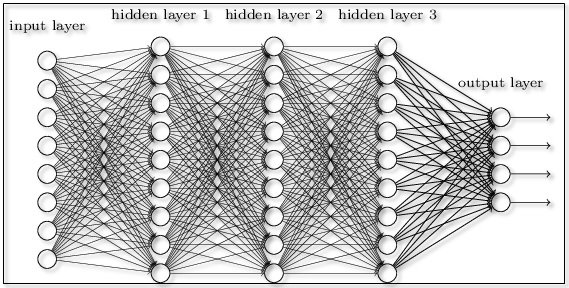
\includegraphics[width=0.6\textwidth]{NN}
    \caption{Αναπαράσταση ενός νευρωνικού δικτύου με τρία κρυφά στρώματα}
    \label{fig:Neural Net}
\end{figure}


 Εφόσον το νευρωνικό δίκτυο σχηματίσει επιτυχώς το στρώμα εξόδου, σκοπός μας είναι να \textit{συγκρίνουμε} τα δεδομένα του στρώματος εξόδου με τις προβλέψεις μας, δηλαδή με τις επιθυμητές τιμές. Αυτό επιτυγχάνεται με τη βοήθεια μιας ειδικής \textit{συνάρτησης κόστους} (Loss Function). Η συνάρτηση αυτή μας βοηθά να ποσοτικοποιήσουμε το σφάλμα ή την απόκλιση των δεδομένων του στρώματος εξόδου σε σχέση με τις επιθυμητές τιμές.

\subsection{Εκπαίδευση ενός Νευρωνικού Δικτύου}
Με τον όρο \textit{εκπαίδευση} του νευρωνικού δικτύου εννοούμε την \textit{ρύθμιση} ή \textit{προσαρμογή} των ειδικών \textit{παραμέτρων} του δικτύου, που ονομάζονται \textit{βάρη} (weights) και \textit{μεροληψίες} (στο εξής bias). Οι παράμετροι αυτοί αρχικοποιούνται τυχαία και με βάση τον αλγόριθμο που θα περιγραφεί παρακάτω προσπαθούμε να βρούμε τις βέλτιστες δυνατές τιμές αυτών.\\

Ας υποθέσουμε ότι έχουμε ένα νευρωνικό δίκτυο με $N$ κρυφά στρώματα, δηλαδή συνολικά το δίκτυο έχει $N+2$ στρώματα. Σε κάθε στρώμα αντιστοιχίζονται δύο \textit{πίνακες}, ο πίνακας των βαρών, $\textbf{W}_i ^j$ και ο πίνακας των biases, $\textbf{b}_k$. Ο δείκτης $i$ αναφέρεται στον $i$ νευρώνα του στρώματος στο οποίο έχει αντιστοιχισθεί ο εκάστοτε πίνακας και ο δείκτης $j$ στον $j$ νευρώνα του ακριβώς επόμενου στρώματος του δικτύου. Ως σύμβαση το στρώμα εισόδου θα έχει $i = in$,  τα κρυφά στρώματα θα έχουν $i,j = 1, \dots , N$ ενώ το στρώμα εξόδου θα έχει $j=out$. Κάθε στοιχείο του πίνακα των βαρών μεταφράζεται ως η συνεισφορά ενός συγκεκριμένου νευρώνα στο υπολογισμό της εξόδου του επόμενου νευρώνα με τον οποίο συνδέεται. Η διαστάσεις του πίνακα των βαρών και των biases καθορίζονται από την διάσταση (τον αριθμό των νευρώνων) των στρωμάτων στα οποία αναφέρεται. Ο πίνακας των biases αντιστοιχίζεται σε όλα τα στρώματα εκτός από το στρώμα εξόδου και έχει διάσταση $1 \times n$, όπου n ο αριθμός των νευρώνων του αντίστοιχου στρώματος. \\

Για παράδειγμα ας υποθέσουμε ότι το στρώμα εισόδου ενός νευρωνικού δικτύου έχει 10 νευρώνες και το αμέσως επόμενο στρώμα, δηλαδή το πρώτο κρυφό στρώμα, έχει 5 νευρώνες (νούμερα πάρα πολύ μικρά για ένα τυπικό νευρωνικό δίκτυο!). Τότε ο πίνακας  $\textbf{W}_{in} ^1$ είναι ο πίνακας των βαρών που δίνει την συνεισφορά των στοιχείων του στρώματος εισόδου στον υπολογισμό της εξόδου των στοιχείων του πρώτου κρυφού στρώματος. Η διάσταση του πίνακα αυτού είναι $5 x 10 = 50$, περιέχει δηλαδή 50 βάρη. Στο κρυφό στρώμα αυτό επίσης αντιστοιχίζονται και 5 βάρη. Άρα προς το παρόν έχουμε 55 μεταβλητές. Τέλος ας υποθέσουμε ότι το νευρωνικό μας δίκτυο έχει μόνο ένα κρυφό στρώμα και το στρώμα εξόδου έχει 3 νευρώνες. Άρα ο πίνακας $\textbf{W}_{N} ^{out}$ θα έχει 30 βάρη και επίσης στο στρώμα εξόδου θα αντιστοιχισθούν 3 βάρη. Συνολικά δηλαδή το νευρωνικό μας δίκτυο αποτελεί μία συνάρτηση $55 + 30 + 3 = 88$ μεταβλητών, οι οποίες όχι μόνο πρέπει να υπολογισθούν αλλά να βρεθεί και η βέλτιστη τιμή αυτών. Όπως είναι προφανές, ακόμα και για ένα πολύ απλό νευρωνικό δίκτυο, η εκπαίδευση αποτελεί μία πολύ περίπλοκη διαδικασία βελτιστοποίησης μιας συνάρτησης πάρα πολλών μεταβλητών. \\

Περιληπτικά η μεθοδολογία της εκπαίδευσης είναι η εξής: Η πληροφορία των δεδομένων εισόδου \textit{προωθείται} μέσα στο νευρωνικό δίκτυο και επεξεργάζεται μέσω της διαδικασίας \textit{feed forward}. Μόλις η πληροφορία φθάσει στο στρώμα εξόδου συγκρίνεται με τις αντίστοιχες επιθυμητές τιμές (που μπορεί να είναι για παράδειγμα πειραματικά δεδομένα ή δικές μας προβλέψεις). Η σύγκριση αυτή γίνεται με την βοήθεια μιας \textit{συνάρτησης κόστους}. \\

\textit{Προώθηση} (Feed Forward) : Το πρώτο στάδιο της εκπαίδευσης ενός νευρωνικού δικτύου είναι η εισαγωγή των δεδομένων μας σε αυτό, μέσω του στρώματος εισόδου, και η επεξεργασία τους από τα κρυφά στρώματα. Η διαδικασία είναι η εξής: \\
Ένα δεδομένο $\textbf{x}_i$ που εξέρχεται από έναν νευρώνα του στρώματος εισόδου πολλαπλασιάζεται με το στοιχείο $\textbf{W}_{i} ^j$ και στο αποτέλεσμα προστίθεται το αντίστοιχο βάρος  $\textbf{b}_i$. Σχηματίζεται έτσι η ποσότητα:
\begin{align*}
\alpha_i ^ j   =  \textbf{W}_i ^j \textbf{x}_i + \textbf{b}_i 
\end{align*}
 $\forall i = 1, 2, \dots, Ν$ όπου Ν ο αριθμός των νευρώνων του στρώματος εισόδου. Η ποσότητα $\alpha_i ^ j$ ονομάζεται \textit{τιμή ενεργοποίησης} (activation value).  Στην συνέχεια αθροίζουμε πάνω στον δείκτη $i$ και παίρνουμε έτσι ένα \textit{σταθμισμένο άθροισμα} των δεδομένων εισόδου. Το άθροισμα αυτό θα αποτελέσει την είσοδο για κάθε νευρώνα του πρώτου κρυφού στρώματος. Όπως προαναφέρθηκε, κάθε νευρώνας ενός κρυφού στρώματος αντιπροσωπεύει μία συνάρτηση ενεργοποίησης. Συνεπώς η έξοδος του κάθε νευρώνα του πρώτου κρυφού στρώματος θα είναι το {κανονικοποιημένο σταθμισμένο άθροισμα}:
\begin{equation}
\displaystyle \sigma \left( \sum_{i=1}^{N} \alpha_i ^ j \right)  =  \sigma \left(\sum_{i=1}^{N} \textbf{W}_i ^j \textbf{x}_i + \textbf{b}_i  \right)
\end{equation}
Από το σημείο αυτό και μέχρι το στρώμα εξόδου η διαδικασία συνεχίζεται με παρόμοιο τρόπο. Στο πρώτo κρυφό στρώμα θα αντιστοιχισθούν οι πίνακες βαρών και biases. Για κάθε νευρώνα του πρώτου κρυφού στρώματος θα σχηματισθεί το σταθμισμένο άθροισμα και τελικά το άθροισμα αυτό θα περάσει σε όλους του νευρώνες του δεύτερου κρυφού στρώματος, όπου και θα δράσει η αντίστοιχη συνάρτηση ενεργοποίησης. Η έξοδος του κάθε νευρώνα του τελευταίου κρυφού στρώματος θα πολλαπλασιασθεί με το αντίστοιχο στοιχείο του τελευταίου πίνακα βαρών, θα προστεθεί το τελευταίο διάνυσμα biases και το τελικό αυτό αποτέλεσμα θα αποτελέσει το στρώμα εξόδου.\\

Στο σημείο αυτό τελειώνει η προώθηση της πληροφορίας κατά μήκος του νευρωνικού δικτύου. Έχοντας το διάνυσμα του στρώματος εξόδου το επόμενο βήμα είναι η 

\section{Συναρτήσεις Ενεργοποίησης}

Οι συναρτήσεις ενεργοποίησης είναι ο τρόπος με τον οποίο η πληροφορία των σημάτων εισόδου περνούν από τον έναν νευρώνα στον επόμενο. Σηματοδοτούν δηλαδή πότε ένας νευρώνας θα "ενεργοποιηθεί" και θα μεταβιβάσει την εκάστοτε πληροφορία. Υπάρχουν πολλές υποψήφιες επιλογές συναρτήσεων ενεργοποίησης και η επιλογή της "καταλληλότερης" συνάρτησης για τον κάθε νευρώνα (η συνηθέστερα για το κάθε κρυφό στρώμα) είναι ως επί το πλείστον εμπειρική και αποτελεί πηγή πολλών ερευνητικών δυνατοτήτων. Για να καταλάβουμε τί είδους συναρτήσεις είναι κατάλληλες για την μεταφορά πληροφορίας μεταξύ των νευρώνων μπορούμε να ξεκινήσουμε μελετώντας ποιες συναρτήσεις \textit{δεν είναι κατάλληληλες} για αυτόν τον σκοπό.\\

Η μελέτη των συναρτήσεων ενεργοποίησης ξεκίνησε με την εξής απλή σκέψη: Εφόσον ένας νευρώνας είτε θα μεταβιβάσει είτε δεν θα μεταβιβάσει την πληροφορία στον επόμενο νευρώνα, τι πιο φυσικό από το να χρησιμοποιήσουμε την \textit{βηματική συνάρτηση} (step function): 

\[ 
\ \sigma(x) = \left\{
\begin{array}{ll}
      1 & , x > 0 \\
      0 & , x < 0 \\
\end{array} 
\right. 
\]

Παρόλο που η παραπάνω συνάρτηση φαίνεται διαισθητικά σωστή, στην πραγματικότητα εμφανίζει πολύ άσχημα αποτελέσματα στην πράξη της εκπαίδευσης των δικτύων. Αυτό οφείλεται στο γεγονός ότι ο ορισμός της παραπάνω συνάρτησης θα επιτρέψει στον νευρώνα είτε να μεταδώσει πλήρως την πληροφορία του είτε καθόλου, ενεργεί δηλαδή με δυαδικό τρόπο. Στην πράξη παρόλα αυτά μία καλή εκπαίδευση θα πρέπει να περιλαμβάνει και "ποσοστά μετάδοσης" πληροφορίας επειδή με αυτόν τον τρόπο η εκπαίδευση του δικτύου \\

Συνεπώς θα πρέπει να επιλέξουμε μία συνάρτηση που να δίνει και ενδιάμεσες τιμές ενεργοποίησης. Η πρώτη σκέψη είναι μία γραμμική συνάρτηση:
\begin{align*}
\sigma (x) = \alpha x
\end{align*}

Μια συνάρτηση τέτοιας μορφής μπορεί να δώσει όντως μια μεγάλη ποικιλία τιμών ενεργοποίησης, οι οποίες τιμές είναι ανάλογες της εκάστοτε εισόδου. Παρόλα αυτά οι γραμμικές συναρτήσεις έχουν δύο σοβαρά μειονεκτήματα. Το πρώτο είναι το γεγονός ότι έχουν \textit{σταθερή βαθμίδα} (ή \textit{κλίση}). Αυτό σημαίνει ότι αν υπάρχει σφάλμα στην πρόβλεψη, δηλαδή η έξοδος του νευρωνικού δικτύου διαφέρει από την επιθυμητή τιμή, τότε η διόρθωση και οι αλλαγές που θα γίνονται με την προς-τα-πίσω μετάδοση θα είναι σταθερές και δεν θα εξαρτώνται από το σφάλμα αυτό. Το δεύτερο μειονέκτημα δεν είναι τόσο προφανές. Αν όλες οι συναρτήσεις ενεργοποίησης επιλεγούν γραμμικές τότε η τελική έξοδος του νευρωνικού δικτύου θα είναι και αυτή μία γραμμική συνάρτηση της εισόδου. Στην ουσία το σύνολο του νευρωνικού δικτύου (που μπορεί να περιέχει μέχρι και δεκάδες κρυφά στρώματα!) θα είναι ισοδύναμο με ένα νευρωνικό δίκτυο με ένα μόνο κρυφό στρώμα, εφόσον η σύνθεση γραμμικών συναρτήσεων είναι μία επίσης γραμμική συνάρτηση. Αυτό στην πράξη σημαίνει χειρότερη εκπαίδευση.\\

Το επόμενο βήμα δεν είναι ιδιαίτερα προφανές. Χρειαζόμαστε μία συνάρτηση που να έχει τουλάχιστον τις εξής ιδιότητες:
\begin{itemize}
  \item Μη-γραμμική
  \item Φραγμένη (προτιμέστερα μεταξύ του 0 και του 1, χωρίς να έχει ιδιαίτερη σημασία)
  \item Να είναι τουλάχιστον μια φορά συνεχώς παραγωγίσιμη 
\end{itemize}

Μία πολύ καλή υποψήφια συνάρτηση είναι η λεγόμενη \textit{λογιστική συνάρτηση}:
\begin{align*}
\sigma(x) = \frac{1}{1+e^{-x}}
\end{align*}

\begin{figure}[h]
    \centering
    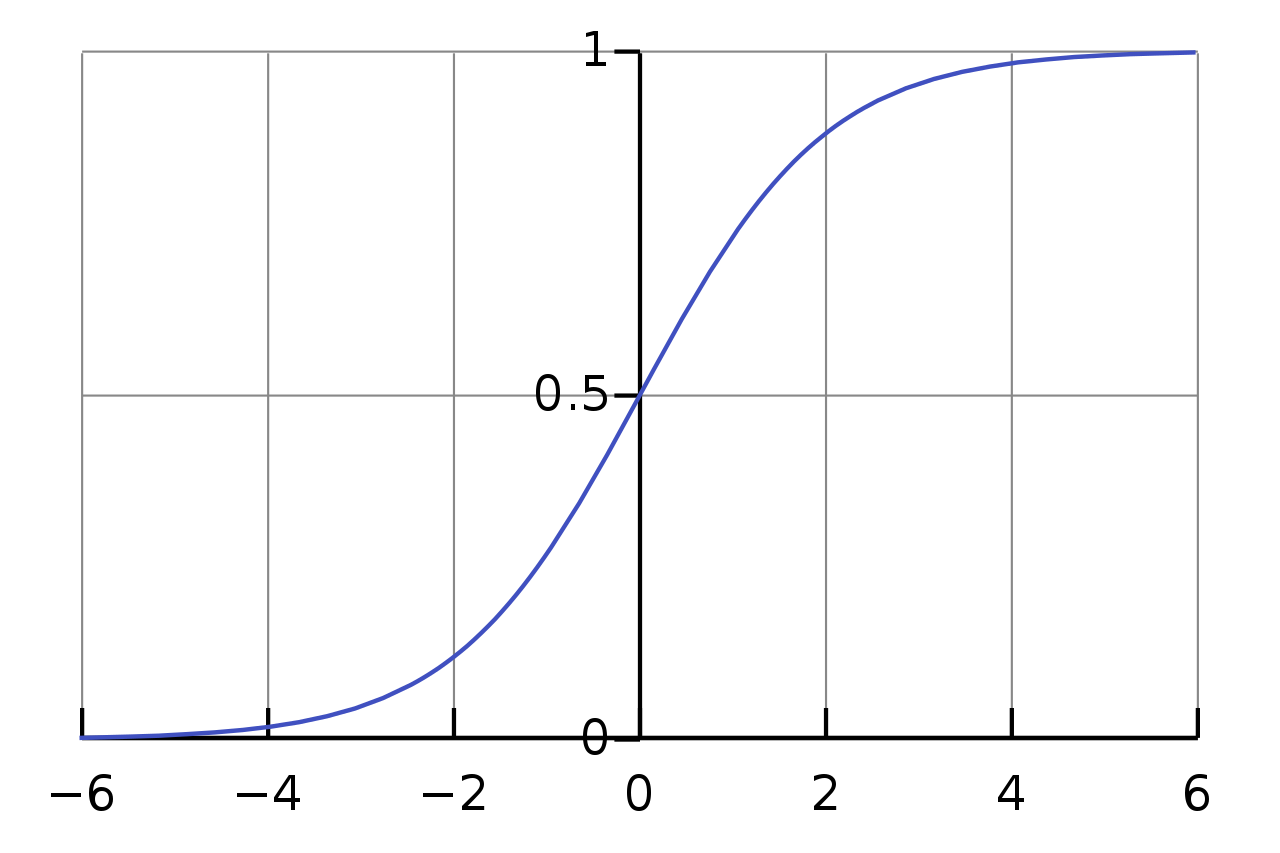
\includegraphics[width=0.6\textwidth]{logcurve}
    \caption{Γραφική παράσταση της λογιστικής συνάρτησης}
    \label{fig:logistic curve}
\end{figure}

Η παραπάνω συνάρτηση έχει όλες τις παραπάνω επιθυμητές ιδιότητες συν άλλη μία η οποία δεν είναι άμεσα προφανής. H λογιστική συνάρτηση έχει κλίση που δίνεται από τον τύπο:
\begin{align*}
\nabla \sigma(x) = \frac{e^x}{(e^x + 1)^2}
\end{align*}

 Στο διάστημα [-2,2] η κλίση της λογιστικής συνάρτησης είναι αρκετά μεγάλη, όπως φαίνεται και από την γραφική της παράσταση. Μεγάλη κλίση σημαίνει πως μικρές μεταβολές των μεταβλητών εισόδου (μικρά Δx) οδηγούν σε μεγάλες μεταβολές των μεταβλητών εξόδου. Υπάρχει δηλαδή αρκετά μεγάλη ευαισθησία σε μικρές διαταραχές του σήματος που εισέρχεται στον νευρώνα και αυτό συνεπάγεται πιο αποδοτική εκπαίδευση με την χρήση της προς-τα-πίσω μετάδοσης. \\

Η λογιστική συνάρτηση είναι όντως μία από τις ευρέως χρησιμοποιούμενες συναρτήσεις ενεργοποίησης στην τεχνολογία των νευρωνικών δικτύων λόγω των προαναφερθέντων ιδιοτήτων της. Στο σημείο αυτό όμως θα πρέπει να αναφερθεί και το μοναδικό μειονέκτημα της εν λόγω συνάρτησης που οφείλεται στην ίδια την φύση της. Παρατηρούμε από την παραπάνω γραφική παράσταση ότι στο σύνολο $[-\infty,-2] \cup [2, +\infty]$ η κλίση της λογιστικής συνάρτησης πρακτικά μηδενίζεται (η συνάρτηση τείνει να γίνει οριζόντια). Παρουσιάζεται δηλαδή το φαινόμενο των \textit{εξαφανισμένων βαθμίδων} (vanishing gradients). Πολύ μικρές βαθμίδες στα διαστήματα αυτά σημαίνει πως μόλις η εκπαίδευση μας οδηγήσει στα "άκρα" της συνάρτησης τότε η εκπαίδευση επιβραδύνεται με πολύ μεγάλο ρυθμό και πρακτικά σταματά.\\

Το επόμενο βήμα αποτελεί μία βελτίωση της λογιστικής συνάρτησης και ονομάζεται \textit{υπερβολική εφαπτομένη}:
\begin{align*}
\sigma(x) = \tanh{x} = \frac{e^x - e^{-x}}{e^x + e^{-x}}
\end{align*}

\begin{figure}[h]
    \centering
    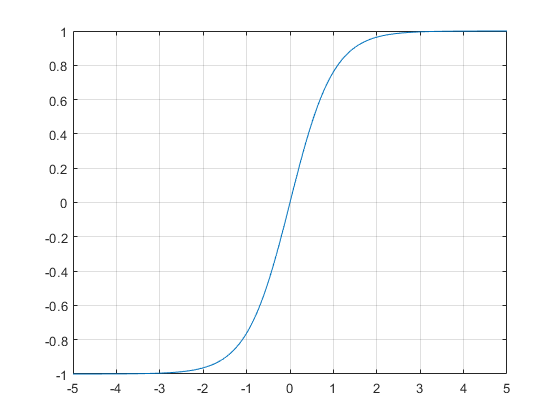
\includegraphics[width=0.6\textwidth]{tanh}
    \caption{Γραφική παράσταση της υπερβολικής εφαπτομένης}
    \label{fig:tanh curve}
\end{figure}

Συγκρίνοντας τις κλίσεις της λογιστικής συνάρτησης και της υπερβολικής εφαπτομένης παρατηρούμε ότι στο κοινό διάστημα [-2,2] η υπερβολική εφαπτομένη έχει μεγαλύτερη κλίση. Κατά τ'άλλα παρουσιάζει τα ίδια μειονεκτήματα και πλεονεκτήματα με την λογιστική συνάρτηση. Η επιλογή ανάμεσα στις δύο αυτές συναρτήσεις εξαρτάται από το πόσο μεγάλες κλίσεις θέλουμε να επιβάλλουμε στο νευρωνικό μας δίκτυο. Αποτελεί προς το παρόν θέμα κυρίως εμπειρικό και εξαρτάται από το εκάστοτε πρόβλημα.\\

Εναλλακτικές επιλογές συναρτήσεων που παρουσιάζουν παρόμοια χαρακτηριστικά με την λογιστική συνάρτηση και την υπερβολική εφαπτομένη είναι οι εξής συναρτήσεις:
\begin{gather*}
f(x) = \arctan{x} \\
f(x) = \frac{x}{1+\abs{x}}\\
f(x) = \frac{x}{\sqrt{1+\alpha x^2}}
\end{gather*}

Όλες οι παραπάνω μη-γραμμικές συναρτήσεις ανήκουν στην ειδικότερη κατηγορία των \textit{σιγμοειδών} συναρτήσεων (sigmoid functions) και είναι η πιο ευρέως χρησιμοποιούμενη κατηγορία συναρτήσεων ενεργοποίησης στα νευρωνικά δίκτυα λόγω των ιδιοτήτων τους. Τα τελευταία χρόνια όμως έχει τεθεί σε εφαρμογή μια συνάρτηση που δεν είναι σιγμοειδής και ονομάζεται \textbf{ReLU} (Rectified Linear Unit). Δίνεται από την σχέση: 
\[ 
\ R(x) = \left\{
\begin{array}{ll}
      x & , x > 0 \\
      0 & , x < 0 \\
\end{array} 
\right. 
\]

Η ReLU μπορεί να ορισθεί και ως R(x) = $\max{(0,x)}$. Παρά το γεγονός ότι με μία πρώτη ματιά η ReLU φαίνεται γραμμική, στην πραγματικότητα δεν είναι. Μια γραμμική απεικόνιση $T : \mathbb{R} \rightarrow \mathbb{R}$ ικανοποιεί τις εξής σχέσεις:
\begin{gather*}
T(x + y) = T(x) + T(y)\\
T(\lambda x) = \lambda x
\end{gather*}

Είναι προφανές ότι η ReLU δεν ικανοποιεί την πρώτη συνθήκη των γραμμικών συναρτήσεων. Ως παράδειγμα έχουμε:\\
$ R(1) = \max{(0,1)} = 1$.
Όμως $1 = 2 - 1$ και αν υποθέσουμε ότι η ReLU είναι γραμμική τότε θα ισχύει ότι:
$R(2 -1) = R(2) + R(-1) = 2 = R(1) = 1$ καί έτσι καταλήγουμε σε άτοπο και άρα στο συμπέρασμα ότι η ReLU δεν είναι γραμμική.

\begin{figure}[h]
    \centering
    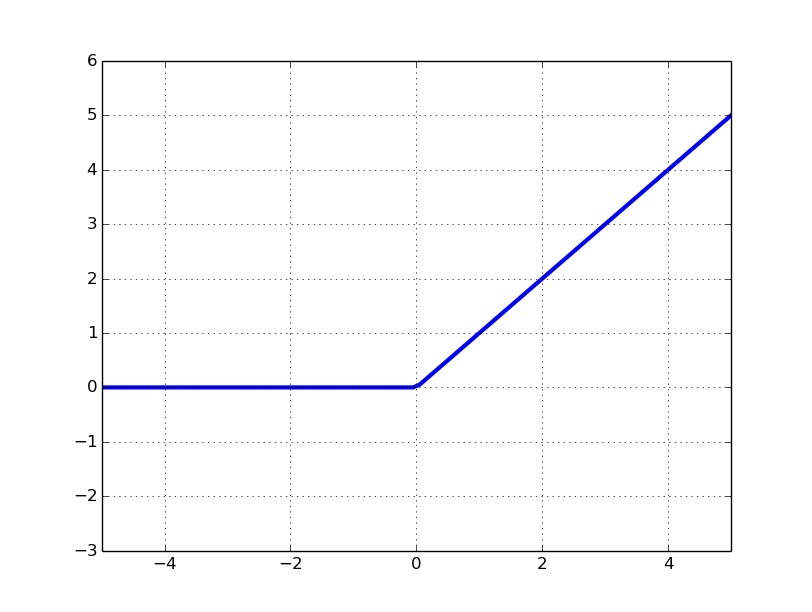
\includegraphics[width=0.6\textwidth]{relu}
    \caption{Γραφική παράσταση της ReLU}
    \label{fig:RELU curve}
\end{figure}

Ένα ενδιαφέρον χαρακτηριστικό της ReLU είναι ότι μπορεί να δράσει πολύ καλά ως συναρτησιακός προσεγγιστής, με την έννοια ότι μπορούμε να προσεγγίσουμε όσο καλά θέλουμε μία συνεχής συνάρτηση με την χρήση γραμμικού συνδυασμού συναρτήσεων ReLU. Πιο φορμαλιστικά, για κάθε $\epsilon > 0$ και για κάθε συνεχή συνάρτηση $f$ υπάρχει ένας φυσικός $Ν$, πραγματικοί αριθμοί $\alpha_i$ και συναρτήσεις ReLU ορισμένες σε κατάλληλο εκάστοτε διάστημα, ώστε :
\begin{align*}
\displaystyle \abs{f - \sum_{i=1}^{N} \alpha_i R_i(x)} < \epsilon
\end{align*}

Στις περισσότερες περιπτώσεις η ReLU χρησιμοποιείται σε συνδυασμό με άλλες συναρτήσεις ενεργοποίησης, συνήθως σιγμοειδείς. Η παρουσία της προσφέρει ένα σημαντικό πλεονέκτημα. Λόγω της μορφής της δεν επιτρέπει σε όλους τους νευρώνες να ενεργοποιηθούν. Αν φανταστούμε ένα νευρωνικό δίκτυο με εκατοντάδες ή και χιλιάδες νευρώνες τότε προφανώς ο υπολογιστικός χρόνος της εκπαίδευσης μπορεί να είναι πολύ μεγάλος για να είναι πρακτικός. Η χρήση της ReLU λοιπόν μας βοηθά να δημιουργήσουμε ένα νευρωνικό δίκτυο πιο αραιό και ανάλαφρο και έτσι να εξοικονομήσουμε πολύτιμο υπολογιστικό χρόνο. Αυτό είναι το μεγάλο πλεονέκτημά της. Το πρόβλημα που δημιουργεί είναι προφανές στο σημείο αυτό και είναι η μηδενική κλίση (δηλαδή τερματισμός της εκπαίδευσης) για αρνητικές τιμές εισόδου. Το πρόβλημα αυτό λύνεται με μικρές παραλλαγές της ReLU που παίρνουν την μορφή:
\[ 
\ R_\epsilon(x) = \left\{
\begin{array}{ll}
      x & , x > 0 \\
      \epsilon x & , x < 0 \\
\end{array} 
\right. 
\]
όπου $\epsilon << 1$. Η μικρή παράμετρος $\epsilon$ μπαίνει έτσι ώστε να υπάρχει μη-μηδενική κλίση για αρνητικές τιμές εισόδου. Τέτοιες παραλλαγές της ReLU είναι γνωστές ως \textbf{Leaky ReLU}.\\

\section{Συναρτήσεις Κόστους}
Η ανάγκη για την ύπαρξη μίας συνάρτησης κόστους στο νευρωνικό δίκτυο έγκειται στο γεγονός ότι χρειαζόμαστε ένα κριτήριο με βάση το οποίο θα γίνει η εκπαίδευση του δικτύου. Οι συναρτήσεις κόστους μας βοηθούν να συγκρίνουμε τις τιμές του στρώματος εξόδου με τις επιθυμητές τιμές (προβλέψεις ή πειραματικά δεδομένα). Είναι δηλαδή ο τρόπος με τον οποίο βοηθούμε τον υπολογιστή να καταλάβει αν η διαδικασία της προώθησης ήταν επιτυχής. Για λόγους που δεν είναι άμεσα προφανείς και σχετίζονται με την διαδικασία του backpropagation οι συναρτήσεις κόστους δεν πρέπει να εξαρτώνται από τις τιμές ενεργοποίησης $\alpha_i ^ j$ αλλά μόνο από τις τιμές του στρώματος εξόδου.\\

\subsection{Συνήθεις συναρτήσεις κόστους}

Μερικές από τις ευρέως χρησιμοποιούμενες συναρτήσεις κόστους είναι οι εξής:\\

\textbf{Συνάρτηση μέσου τετραγωνικού σφάλματος} (Mean Square Error Function):
\begin{align*}
\displaystyle C = \frac{1}{n} \sum_{i=1}^{n} (y_i - \hat{y}_i)^2
\end{align*}
όπου $y_i$ οι τιμές του στρώματος εξόδου του δικτύου και $\hat{y}_i$ οι προβλέψεις μας με τις οποίες τις συγκρίνουμε. Η συνάρτηση αυτή χρησιμοποιείται ευρέως σε προβλήματα παλινδρόμησης (regression) όμως έχει ένα σοβαρό πρόβλημα. Σε περίπτωση που υπάρχουν δεδομένα (παρατηρούμενες τιμές) που απέχουν πολύ από όλα τα υπόλοιπα, τα λεγόμενα outliers, τότε η εφαρμογή της συνάρτησης τετραγωνικού σφάλματος μπορεί να έχει πολύ μεγάλα σφάλματα στους υπολογισμούς. Για τον σκοπό αυτό επινοήθηκε η συνάρτηση σφάλματος κατά Huber. \\

$(wiki και https://ml-cheatsheet.readthedocs.io/en/latest/loss_functions.html(εδώ υπάρχει δίεση)kullback-leibler)$
\textbf{Συνάρτηση Huber} (Huber Loss):
\[ 
\ C = \left\{
\begin{array}{ll}
    \displaystyle \frac{1}{2} \sum_{i} (y_i - \hat{y}_i)^2 & , \abs{y_i - \hat{y}_i} \leq \delta \forall i\\
    \displaystyle \delta \sum_{i} \abs{y_i - \hat{y}_i} - \frac{1}{2} \delta ^ 2& ,otherwise\\
\end{array} 
\right. 
\]
Η συνάρτηση Huber είναι πολύ λιγότερο ευαίσθητη σε outliers.\\

\textbf{Συνάρτηση Cross Entropy}:
\begin{align*}
\displaystyle C = -\sum_{i=1}^{n} y_i \log{\hat{y}_i}
\end{align*}
Η Cross Entropy αποτελεί μια από τις σημαντικότερες συναρτήσεις για το κλάδο τον Μαθηματικών με όνομα Θεωρία Πληροφορίας.\\

Όλες οι μορφές των παραπάνω συναρτήσεων αφορούν φυσικά διακριτό χώρο δειγματοληψίας. Αν οι κατανομές μας αποτελούν συνεχείς συναρτήσεις τότε το άθροισμα αντικαθιστάται με ολοκλήρωμα.\\

\subsection{Κανονικοποίηση Κόστους}
[ubc 2018 february, deeplearningbook]


$[ΑΜ221_lecture9.pdf, conv_opt.pdf]$
\section{Κατάβαση Βαθμίδας (Gradient Descent)}
\subsection{Το πρόβλημα και ο αλγόριθμος}
Η διαδικασία του Gradient Descent είναι ένας αλγόριθμος με τον οποίο μπορούμε να βρούμε ένα \textit{τοπικό ακρότατο} μιας πολυμεταβλητής συνάρτησης. Η ιδέα πίσω από τον αλγόριθμο είναι απλή. Ξεκινώντας από ένα αυθαίρετο σημείο πάνω στην (υπερ)επιφάνεια που ορίζει η συνάρτηση μας τότε αν θέλουμε να κάνουμε ανάβαση της επιφάνειας, δηλαδή να πάμε προς το πιο κοντινό μέγιστο, τότε θα πρέπει να ακολουθήσουμε την κατεύθυνση που ορίζει η \textit{βαθμίδα} (gradient) της συνάρτησης στο σημείο αυτό. Αυτό είναι και το φυσικό νόημα του gradient. Σε κάθε σημείο της επιφάνειας μας λέει προς τα που πρέπει να κινηθούμε έτσι ώστε να έχουμε την μεγαλύτερη αύξηση ή \textit{κλίση}. Συνεπώς, αν επιθυμούμε να κάνουμε κατάβαση της επιφάνειας τότε θα πρέπει να ακολουθήσουμε πορεία \textit{αντίθετη της βαθμίδας}. Σε ακριβώς έγκειται ο αλγόριθμος του gradient descent, στην επικαιροποίηση ενός τυχαίου σημείου της επιφάνειας με βήμα ανάλογο της βαθμίδας.\\

Ας υποθέσουμε λοιπόν ότι μας δίνεται ένα συνεκτικό ανοιχτό χωρίο $D \subset \mathbb{R}^d$ και μία πραγματική κυρτή συνάρτηση $f \in C^1 (D)$, η οποία θα αποκαλείται \textit{αντικειμενική συνάρτηση} (objective function)
\begin{align*}
f : D \rightarrow \mathbb{R}
\end{align*}
την οποία επιθυμούμε να ελαχιστοποιήσουμε. Ψάχνουμε δηλαδή ένα $\textbf{x}^*$, τέτοιο ώστε:
\begin{align*}
\textbf{x}^* =  \operatorname*{argmin}_{\textbf{x} \in D} f(\textbf{x})
\end{align*}
Προφανώς επίσης θα ισχύει
\begin{align*}
\nabla f(\textbf{x}^*) = 0
\end{align*}

Ο αλγόριθμος απαιτεί να του ορίσουμε το αρχικό σημείο πάνω στην επιφάνεια από το οποίο θα αρχίσει η κατάβαση (ή η ανάβαση), το \textit{βήμα επικαιροποίησης} $t_k$ και ένα \textit{όριο} (threshold) το οποίο θα καθορίσει πότε θα σταματήσει ο αλγόριθμος. Συνοπτικά ο αλγόριθμος gradient descent φαίνεται στον παρακάτω πίνακα. \\


\begin{tabular}{ |p{13cm}}
 \hline
 \multicolumn{1}{|c|}{\textbf{Αλγόριθμος Gradient Descent}} \\
 \hline
1: Αρχικοποίηση τυχαίου σημείου $\textbf{x}^{(0)}$, βήματος $t_0$ και threshold $\epsilon$ \\
2: \textbf{while} $||\nabla f(\textbf{x}^{(k)})|| \geq \epsilon$ \textbf{do} :  \\
3: $\textbf{x}^{(k+1)} = \textbf{x}^{(k)} - \tau \nabla f(\textbf{x}^{(k)})$\\
4: $k \leftarrow k + 1$ \\
5: \textbf{end while}  \\
6: \textbf{return} $\textbf{x}^{(k)}$\\
\hline
\end{tabular}\\

Μερικά σχόλια για τον αλγόριθμο και τις παραμέτρους του. Καταρχάς ο παραπάνω αλγόριθμος αναφέρεται σε προβλήματα βελτιστοποίησης \textit{χωρίς περιορισμούς}, δηλαδή θεωρούμε ότι όλα τα σημεία του χώρου που ορίζονται από την επιφάνεια που ορίζει η αντικειμενική συνάρτηση είναι προσβάσιμα. Ο αλγόριθμος τροποποιείται για προβλήματα που περιέχουν περιορισμούς όμως έχει την ίδια επιτυχία.\\

Το βήμα επικαιροποίησης $\tau$  μπορεί να είναι είτε ένας σταθερός αριθμός είτε να εξαρτάται από το βήμα στο οποίο βρισκόμαστε. Η δεύτερη περίπτωση είναι πιο αποδοτική αν το βήμα επιλεγεί με έναν σχετικά έξυπνο τρόπο. Το κόστος φυσικά είναι αρκετά μεγαλύτεροι υπολογιστικοί χρόνοι. Η λογική πίσω από την επιλογή του βήματος είναι η σκέψη ότι θέλουμε να ελαχιστοποιεί την αντικειμενική μας συνάρτηση σε μια περιοχή του βήματος στο οποίο πρόκειται να βρεθούμε μετά από το εκάστοτε βήμα. Σε μαθηματικούς όρους, το \textit{βέλτιστο βήμα} $t_k ^ *$ θα ικανοποιεί:
\begin{align*}
t_k ^ * = \operatorname*{argmin}_{t \geq 0} f(\textbf{x}^{(k+1)}) = \operatorname*{argmin}_{t \geq 0} f(\textbf{x}^{(k)} - t \nabla f(\textbf{x}^{(k)})
\end{align*}

Φυσικά είναι εξαιρετικά λίγες οι περιπτώσεις όπου το βήμα αυτό μπορεί να υπολογισθεί αναλυτικά μιας και στις περισσότερες εφαρμογές οι αντικειμενικές συναρτήσεις είναι μέχρι και δεκάδων μεταβλητών.\\

Το όριο $\epsilon$ είναι το κριτήριο τερματισμού του αλγορίθμου και είναι ένας πραγματικός αριθμός πολύ μικρότερος της μονάδας και φυσικά θετικός. Όταν η νόρμα (δηλαδή το μέγεθος) της βαθμίδας, $||\nabla f||$, πέσει κάτω από $\epsilon$ μετά την κ-οστή επανάληψη τότε αυτό σημαίνει ότι σε περιοχή του σημείου $\textbf{x}^{(k)}$ η κλίση της συνάρτηση είναι σχεδόν μηδενική και άρα ως γνωστόν θα είμαστε πολύ κοντά στο ακρότατο. Θεωρητικά μπορούμε να προσεγγίσουμε το ακρότατο αυτό όσο καλά θέλουμε μικραίνοντας όλο και πιο πολύ το $\epsilon$.\\

Φυσικά, επειδή καταφέραμε να βρούμε έναν τρόπο να προσεγγίσουμε ένα τοπικό ακρότατο μίας συνάρτησης δεν σημαίνει ότι μπορούμε πάντα να εντοπίσουμε το \textit{ολικό ελάχιστο} μιας συνάρτησης. Στην πραγματικότητα, ο προσδιορισμός του ολικού ελαχίστου μια πολυμεταβλητής συνάρτησης είναι ένα υπέρμετρα δύσκολο μαθηματικό πρόβλημα. Για τον λόγο αυτό στις περισσότερες εφαρμογές η εύρεση ενός τοπικού ακροτάτου της αντικειμενικής μας συνάρτησης θεωρείται επιτυχία. \\

\subsection{Σύγκλιση του αλγορίθμου Gradient Descent}
Ένα εύλογο ερώτημα που προκύπτει είναι κατά πόσο ο αλγόριθμος gradient descent δουλεύει, δηλαδή κατά πόσο συγκλίνει. Η απάντηση δεν είναι απλή και χρειαζόμαστε, μεταξύ άλλων, τον παρακάτω ορισμό:\\

\textbf{Ορισμός}: Έστω ένα κυρτό σύνολο $D \subset \mathbb{R}^d$, μία κυρτή συνάρτηση $f : D \rightarrow \mathbb{R}$. Η $f$ θα λέγεται \textbf{ισχυρώς κυρτή} (strongly convex) αν υπάρχει θετικός πραγματικός αριθμός m τέτοιος ώστε για κάθε $x,y \in D$:
\begin{align*}
\langle \nabla f(x) - \nabla f(y), x - y \rangle \geq m \parallel x - y \parallel ^ 2
\end{align*}
όπου $\parallel \cdot \parallel$ μία οποιαδήποτε νόρμα. Αποδεικνύεται ότι η παραπάνω ανισότητα ισοδυναμεί με την ύπαρξη θετικών πραγματικών αριθμών m και M για τους οποίους ισχύει:
\begin{align*}
mI \leq \mathcal{H}_f (\textbf{x}) \leq MI
\end{align*}
όπου $\mathcal{H}_f (\textbf{x})$ ο εσσιανός πίνακας της $f$ στο \textbf{x} και I ο μοναδιαίος πίνακας. Σημειώνεται ότι για δύο πίνακες A και B ίδιων διαστάσεων $A \geq B$ σημαίνει ότι ο πίνακας Α - B είναι θετικά ημι-ορισμένος.  Μπορούμε έυκολα να δείξουμε ότι μία ισχυρώς κυρτή συνάρτηση είναι και αυστηρά κυρτή. Παίρνοντας το ανάπτυγμα Taylor δεύτερης τάξης για την $f$ έχουμε ότι για $x,y \in D$ μπορούμε να βρούμε ένα $z \in [x, y]$ τέτοιο ώστε:
\begin{align*}
f(y) = f(x) + \nabla f(x) ^ \intercal (y - x) + \frac{1}{2} (y - x) ^ \intercal \mathcal{H}_f (y - x)
\end{align*}
και λόγω της παραπάνω διπλής ανισότητα παίρνουμε:
\begin{align*}
f(y) \geq f(x) + \nabla f(x) ^ \intercal (y - x) + \frac{m}{2} \parallel y - x \parallel ^ 2
\end{align*}
και επειδή $\frac{m}{2} \parallel y - x \parallel ^ 2 > 0$:
\begin{align*}
f(y) > f(x) + \nabla f(x) ^ \intercal (y - x)
\end{align*}
Έχοντας τώρα την ιδιότητα της ισχυρής σύγκλισης παίρνουμε το εξής θεώρημα:\\

\textbf{Θεώρημα}: Έστω $ f : D \rightarrow \mathbb{R}$ μία ισχυρώς κυρτή συνάρτηση με παραμέτρους m και Μ, όπως και στην παραπάνω διπλή ανισότητα, και $\alpha^* = \min_{\textbf{x} \in D} f(\textbf{x})$. Τότε για κάθε $\epsilon > 0$ μπορούμε να πετύχουμε $f(\textbf{x}^{(k^*)}) - \alpha^* \leq \epsilon$ μετά από $k^*$ επαναλήψεις για κάποιο $κ^*$ που ικανοποιεί:
\begin{align*}
k^* \geq \frac{\log \left( \frac{f(\textbf{x}^{(0)}) - \alpha^*}{\epsilon}\right)}{\log \left( \frac{1}{1 - \frac{m}{M}} \right)}
\end{align*}

Το παραπάνω θεώρημα μας εξασφαλίζει ότι μετά από έναν αριθμό επαναλήψεων που εξαρτάται από την φύση της ίδιας της συνάρτησης (τις σταθερές m και Μ) αλλά και από την ακρίβεια που επιθυμούμε μπορούμε να φτάσουμε όσο κοντά θέλουμε στο ακρότατο της $f$. Προφανώς όταν $\epsilon \rightarrow 0$ τότε $k^* \rightarrow +\infty$. Επίσης παρατηρούμε ότι καθώς $m \rightarrow M$ απαιτούνται όλο και λιγότερες επαναλήψεις για να συγκλίνει ο αλγόριθμος.\\

Προφανώς ο ρόλος του αλγορίθμου του gradient descent στα πλαίσια των νευρωνικών δικτύων είναι η ελαχιστοποίηση των συναρτήσεων κόστους ως προς τις παραμέτρους του δικτύου, δηλαδή τα βάρη και τα biases. Συνεπώς ένα κρίσιμο βήμα της εκπαίδευσης είναι ο υπολογισμός των βαθμίδων της συνάρτησης κόστους ως προς όλες αυτές τις παραμέτρους ξεχωριστά. Στο σημείο αυτό όμως, έχοντας αρχίσει να εφαρμόζουμε τον αλγόριθμο gradient descent, παρατηρούμε ότι παρουσιάζεται ένα μείζονος σημασίας πρόβλημα και αυτό είναι οι τεράστιοι υπολογιστικοί χρόνοι που απαιτούνται για να τερματίσει ο αλγόριθμος. Όπως είδαμε και στην ενότητα \textbf{4.1} μία τυπική συνάρτηση κόστους έχει την γενική μορφή:\\
\begin{align*}
\displaystyle \textbf{J(\theta)} = \frac{1}{n} \sum_{i=1}^{n} \mathcal{L}(\textbf{\theta})
\end{align*}
όπου $\mathcal{L}$ μία συνάρτηση σφάλματος (π.χ. η διαφορά των τετραγώνων) και \textbf{\theta} το διάνυσμα των παραμέτρων ως προς τις οποίες επιθυμούμε να γίνει η βελτιστοποίηση, δηλαδή η εύρεση των σημείων μηδενισμού της βαθμίδας
\begin{align*}
\displaystyle \nabla_{\textbf{\theta}} \textbf{J(\theta)} \ = \frac{1}{n} \sum_{i=1}^{n} \nabla_{\textbf{\theta}} \mathcal{L}(\textbf{\theta})
\end{align*}
Ο υπολογιστικός χρόνος (ή υπολογιστικό κόστος) της παραπάνω πράξης είναι $\mathcal{O}(n)$. Συνεπώς όταν ο αριθμός των δεδομένων, $n$, γίνεται πάρα πολύ μεγάλος και ειδικά αν το πρόβλημά μας αφορά μη-κυρτή βελτιστοποίηση τότε η εφαρμογή του αλγορίθμου gradient descent είναι απολύτως μη-πρακτική. Φαίνεται λοιπόν ότι χρειαζόμαστε μία τροποποίηση προκειμένου να είμαστε σε θέση να λύσουμε αποδοτικά ένα πρόβλημα μηχανικής μάθησης.

\subsection{Στοχαστικός Αλγόριθμος Gradient Descent και Mini-Batch Gradient Descent}
[deeplearningbook, $https://gluon.mxnet.io/chapter06_optimization/gd-sgd-scratch.html$, $https://towardsdatascience.com/difference-between-batch-gradient-descent-and-stochastic-gradient-descent-1187f1291aa1$]\\
Ο αλγόριθμος του στοχαστικού gradient descent είναι μία επέκταση του κανονικού αλγορίθμου που περιγράφηκε στην ενότητα \textbf{5.1}. Η ανάγκη της ανάπτυξης του εν λόγω αλγορίθμου έγκειται στις δυσκολίες που παρουσιάζονται στην εφαρμογή του απλού gradient descent όταν ο αριθμός των δεδομένων εκπαίδευσης είναι πάρα πολύ μεγάλος. Πιο συγκεκριμένα, όπως είδαμε στην ενότητα \textbf{4.1}, οι συναρτήσεις κόστους αποτελούν αθροίσματα (τετραγωνικών ή και άλλου είδους) σφαλμάτων μεταξύ των δεδομένων εξόδου και των προβλέψεών μας. Όταν έχουμε στην διάθεσή μας έναν υπερβολικά μεγάλο αριθμό δεδομένων (της τάξεως των εκατομμυρίων) τότε προφανώς ένα μονάχα βήμα του αλγορίθμου gradient descent απαιτεί πάρα πολύ μεγάλο υπολογιστικό χρόνο.\\

Η καρδιά του στοχαστικού gradient descent είναι η εφαρμογή του κλασσικού gradient descent με την παραλλαγή ότι σε κάθε επανάληψη θα υπολογίζουμε την βαθμίδα \textit{για ένα μόνο δεδομένο}. Με άλλα λόγια, στην i-οστή επανάληψη του αλγορίθμου, αντί να υπολογίσουμε την βαθμίδα $\displaystyle \sum_{i=1}^{n} \nabla_{\theta} \mathcal{L}_i$ θα πρέπει μόνο να υπολογίσουμε την βαθμίδα $\nabla_{\theta} \mathcal{L}_i$. Με την μέθοδο αυτή ο υπολογιστικός χρόνος μειώνεται σημάντικα αφού σε κάθε επανάληψη θα πρέπει να υπολογίσουμε πολύ πιο απλές βαθμίδες σε σχέση με την κλασσική έκδοση του αλγορίθμου.\\

Μία μικρή παραλλαγή του στοχαστικού gradient descent είναι ο λεγόμενος αλγόριθμος \textit{mini-batch gradient descent}. Στην περίπτωση αυτή κάνουμε μία τυχαία επιλογή \textit{τεμαχίων} (mini-batches) σταθερού μεγέθους $|\mathcal{B}|$ από τα δεδομένα μας και εφαρμόζουμε τον αλγόριθμο gradient descent σε αυτά. Σε κάθε επανάληψη δηλαδή θα πρέπει να υπολογισθεί η βαθμίδα
\begin{align*}
\displaystyle \nabla_{\textbf{\theta}} \textbf{J(\theta)} \ = \frac{1}{|\mathcal{B}|} \sum_{i=1}^{|\mathcal{B}|} \nabla_{\textbf{\theta}} \mathcal{L}(\textbf{\theta})_i
\end{align*}
Ο υπολογιστικός χρόνος σε αυτήν την περίπτωση είναι $\mathcal{O}(\mathcal{B})$.


[deeplearningbook.pdf]
\section{Προς-τα-πίσω Διάδοση (Back Propagation)}

Έχοντας τώρα τον αλγόριθμο που θα χρησιμοποιήσουμε (gradient descent) για την ελαχιστοποίηση του κόστους θα πρέπει να σκεφτούμε πώς θα υπολογίσουμε τις μερικές παραγώγους (βαθμίδες) που απαιτεί. Η μεθοδολογία υπολογισμού αυτών των μερικών παραγώγων ονομάζεται \textit{προς-τα-πίσω διάδοση ή back-propagation} και επιτρέπει την ροή πληροφορίας που παίρνουμε από τη συνάρτηση κόστους \textit{προς τα πίσω} κατά μήκος του νευρωνικού δικτύου. Η ροή αυτή μοντελοποιείται με βάση τον γνώστο από τον Μαθηματικό Λογισμό \textit{κανόνα της αλυσίδας}. Έστω $\textbf{x} \in \mathbb{R}^m$, $\textbf{y} \in \mathbb{R}^n$, $g : \mathbb{R}^m \rightarrow \mathbb{R}^n$ και $f : \mathbb{R}^n \rightarrow \mathbb{R}$. Απαιτούμε $g \in C^1 (\mathbb{R}^m)$ και $f \in C^1 (\mathbb{R})^n$. Αν $\textbf{y} = g(\textbf{x})$ και $z = f(\textbf{y})$ τότε:
\begin{align*}
\displaystyle \pdv{z}{x_i} = \sum_{j} \pdv{z}{y_j} \pdv{y_j}{x_i} =  \sum_{j} \pdv{z}{y_j} \mathcal{J}_{ij}
\end{align*}
όπου $\mathcal{J}_{ij}$ ο \textit{Ιακωβιανός πίνακας} της $g$.




\section{Ενισχυτική Μάθηση}
\subsection{Διαδικασία Απόφασης κατά Markov}

[DRL.pdf] Η \textit{Ενισχυτική Μάθηση} (Reinforcement Learning) είναι ένας κλάδος της μηχανικής μάθησης που λειτουργεί μέσω ακολουθιακής λήψης αποφάσεων. Ο μαθηματικός φορμαλισμός της ενισχυτικής μάθησης περιλαμβάνει τη λεγόμενη \textit{Διαδικασία Απόφασης κατά Markov} (Markov Decision Process). Η μεθοδολογία αυτή μελετά την αλληλεπίδραση ενός \textit{πράκτορα} (agent) με το \textit{περιβάλλον} (enviroment) στο οποίο ανήκει. Σκοπός του πράκτορα είναι εν τέλει να μεταβεί σε μία επιθυμητή τελική \textit{κατάσταση} (state). Πιο συγκεκριμένα, ο πράκτορας είναι σε θέση να επιλέξει μία από τις επιτρεπόμενες \textit{δράσεις} (actions) έτσι ώστε να μεταβεί από την τρέχουσα κατάσταση στην οποία βρίσκεται στην επόμενη. Αφού γίνει αυτή η μετάβαση, ο πράκτορας αξιολογείται μέσω μίας \textit{αμοιβής} (reward). Η αμοιβή αυτή στα πλαίσια της μηχανικής μάθηση είναι αυθαίρετη. Για παράδειγμα, κάθε φορά που ο πράκτορας μεταβαίνει σε μία κατάσταση από την οποία δεν επωφελείται ή απομακρύνεται από την τελική επιθυμητή κατάσταση, τότε δίνουμε αμοιβή 0 ή -1 ενώ κάθε φορά που ο πράκτορας μεταβαίνει σε μία κατάσταση που τον φέρνει πιο κόντα στον τελικό στόχο τότε δίνουμε αμοιβή +1. Για μερική ευκολία στην κατανόηση, μπορούμε να κάνουμε τον εξής παραλληλισμό: \\

Ας φανταστούμε ότι ο πράκτορας είναι, για παράδειγμα, ένα κατοικίδιο το οποίο θέλουμε να σωφρονίσουμε. Κάθε φορά που το κατοικίδιο δεν ησυχάζει όταν του το ζητάμε τότε δεν του δίνουμε σημασία (αμοιβή 0) ή το βγάζουμε έξω από το σπίτι (αμοιβή -1). Σε αντίθετη περίπτωση, όταν το κατοικίδιο αρχίσει να καταλαβαίνει την εντολή μας και ησυχάζει όταν του το ζητάμε τότε το επιβραβεύουμε με κάτι που του αρέσει (π.χ. ένα φαγητό που του αρέσει, αμοιβή +1). Το παράδειγμα αυτό είναι εξαιρετικά απλοϊκό αφού εδώ οι πιθανές καταστάσεις είναι μόνο δύο (το κατοικίδιο είναι είτε ήσυχο είτε όχι) και οι πιθανές δράσεις είναι επίσης δύο (είτε να υπακούσει στην εντολή μας είτε όχι). Η βασική ιδέα όμως είναι αυτή. \\

Έχοντας τα παραπάνω, είμαστε έτοιμοι τώρα να διατυπώσουμε πιο φορμαλιστικά μία Διαδικασία Απόφασης κατά Markov (στο εξής MDP). Αποτελεί μία διακριτή στοχαστική διαδικασία ελέγχου και διατυπώθηκε για πρώτη φορά από τον Richard Ernest Bellman. Η ιδέα αυτή, παρόλο που προς το παρόν θα ορισθεί σε διακριτά σύνολα, μπορεί να επεκταθεί και σε συνεχείς χώρους, όπως θα γίνει σε μετέπειτα στάδιο.\\

\textbf{Ορισμός}: Μία (διακριτή) \textit{Διαδικασία Απόφασης κατά Markov} (MDP) είναι μία πεντάδα $(\mathcal{S}, \mathcal{A}, \mathcal{P}, R, \gamma)$ όπου:
\begin{itemize}
  \item $\mathcal{S}$ ο \textit{Χώρος Καταστάσεων} (State Space)
  \item $\mathcal{A}$ ο \textit{Χώρος Δράσεων} (Action Space)
  \item $\mathcal{P}$ :  $\mathcal{S} \times  \mathcal{S} \times  \mathcal{A} \rightarrow [0,1]$ η φραγμένη \textit{συνάρτηση μετάβασης} (transition function) που περιλαμβάνει το σύνολο των δεσμευμένων πιθανοτήτων μετάβασης μεταξύ των καταστάσεων.
  \item $R :  \mathcal{S} \times  \mathcal{S} \times  \mathcal{A} \rightarrow  \mathcal{R}$ η \textit{συνάρτηση αμοιβής} (reward function) και  $\mathcal{R}   \subset \mathbb{R}^+$
  \item $\gamma \in [0,1)$ ο \textit{παράγοντας προεξόφλησης} (discount factor). 
\end{itemize}

Σε κάθε χρονικό βήμα $t$ η πιθανότητα μετάβασης από την κατάσταση $s_t$ στην επόμενη κατάσταση, $s_{t+1}$, μέσω την λήψης της απόφασης $\alpha_t$ δίνεται από την συνάρτηση $\mathcal{P}(s_t, s_{t+1},  \alpha_t)$, ενώ η αντίστοιχη αμοιβή από την συνάρτηση R($s_t$,$s_{t+1}$, $\alpha_t$). Όσον αφορά την συνάρτηση μετάβασης, θεωρούμε ότι μία MDP ικανοποιεί την \textit{ιδιότητα Markov}. Στην ουσία, η πιθανότητα να μεταβούμε σε μια επόμενη κατάσταση, $s_{t+1}$, εξαρτάται μόνο από το άμεσο παρελθόν της διαδικασίας, δηλαδή μόνο από την κατάσταση του προηγούμενου χρονικού βήματος, $s_t$. Ο ρόλος του παράγοντα προεξόφλησης $\gamma$ θα αναλυθεί παρακάτω.  \\

Διαγραμματικά, μία MDP φαίνεται στο παρακάτω σχήμα:\\
\begin{figure}[h]
    \centering
    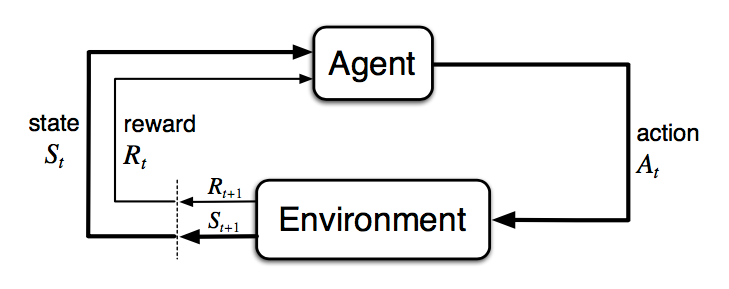
\includegraphics[width=0.6\textwidth]{mdp}
    \caption{Μία τυπική Διαδικασία Απόφασης κατά Markov}
    \label{fig:mdp}
\end{figure}

Όπως είναι προφανές, σκοπός μίας MDP είναι να μεταβούμε σε μία επιθυμητή τελική κατάσταση αρχίζοντας από μία δεδομένη, γνωστή κατάσταση. Εφόσον οι μεταβάσεις μεταξύ των καταστάσεων γίνεται μέσω των διαθέσιμων δράσεων σημαίνει ότι, ιδανικά, θα πρέπει να προσδιορίσουμε μία συνάρτηση:
\begin{align*}
\mathcal{\pi} : \mathcal{S} \rightarrow \mathcal{A}
\end{align*}

Η συνάρτηση $\mathcal{\pi}$ ονομάζεται \textit{πολιτική ή στρατηγική} (policy) και θα είναι στην ουσία ο οδηγός του πράκτορα δια μέσου της MDP, δηλαδή θα είναι ένας κανόνας επιλογής δράσης σε μία δεδομένη κατάσταση. Θα εξετάσουμε αργότερα με ποια κριτήρια θα πρέπει να προσδιορισθεί η συνάρτηση αυτή. Επίσης κρίνεται σκόπιμο να αναφερθεί ότι οι συναρτήσεις πολιτικής διακρίνονται σε \textit{ντετερμινιστικές}, όπως η παραπάνω, και σε \textit{μη-ντετερμινιστικές}. Στην δεύτερη περίπτωση οι συναρτήσεις πολιτικής ορίζονται ως:
\begin{align*}
\mathcal{\pi} : \mathcal{S} \times \mathcal{A} \rightarrow [0,1]
\end{align*}

 Οι ντετερμινιστικές συναρτήσεις πολιτικής καθορίζουν πλήρως ποια δράση είναι η καταλληλότερη για την δεδομένη κατάσταση, ενώ οι μη-ντετερμινιστικές συναρτήσεις πολιτικής έχουν στοχαστική λειτουργία και μας δίνουν την πιθανότητα να επιλεγεί μία δράση $\alpha$ όταν ο πράκτορας βρίσκεται σε μία κατάσταση $s$.\\

Τώρα που έχουμε έναν στόχο, δηλαδή τον προσδιορισμό της συνάρτησης $\mathcal{\pi}$, θα πρέπει να σκεφτούμε με τι κριτήρια θα την επιλέξουμε. Για τον σκοπό αυτό χρειαζόμαστε τους εξής ορισμούς:\\

\textbf{Ορισμός} : Το \textit{Αναμενόμενο Κέρδος} (Expected Return) μίας MDP ορίζεται ως:
\begin{align*} 
\displaystyle G_t = \sum_{k=0}^{+\infty} \gamma^k R_{t+k+1}
\end{align*}
όπου $R_t = R(s_t, \alpha, s_{t+1})$. Είναι δηλαδή η τιμή του \textit{προεξοφλημένου} κέρδους (discounted reward) που λαμβάνει ο πράκτορας ξεκινώντας από μία κατάσταση $s_t$ και ακολουθώντας μία συγκεκριμένη δράση. \\

Ο παράγοντας $\gamma$ παίζει διπλό ρόλο. Καταρχάς, το γεγονός ότι είναι μία σταθερή τιμή μικρότερη της μονάδας επιτρέπει στο παραπάνω άπειρο άθροισμα να συγκλίνει ευκολότερα, εφόσον στις περισσότερες περιπτώσεις η συνάρτηση αμοιβής είναι και αυτή μια φραγμένη συνάρτηση. Η φυσική του σημασία είναι η εξής: Καθώς $\gamma \rightarrow 0$ (και κάνοντας τη σύμβαση ότι $0^0 = 1$) παρατηρούμε ότι όλοι οι όροι του αθροίσματος πέραν του $R_{t+1}$ μηδενίζονται. Αυτό σημαίνει ότι ο πράκτορας δρα "μυωπικά", δηλαδή σκοπός του είναι να βρει τρόπο να πάρει το μέγιστο δυνατό κέρδος στο επόμενό του βήμα, χωρίς να έχει μακροπρόθεσμες βλέψεις. Εν αντιθέσει, καθώς $\gamma \rightarrow 1$ ο πράκτορας δίνει όλο και περισσότερο βάρος σε μελλοντικές αμοιβές και δρά έτσι ώστε να έχει μακρυπρόθεσμα το μέγιστο κέρδος.\\

Τέλος δεν είναι δύσκολο να δείξει κανείς ότι:
\begin{align*}
G_t = R_{t+1} + \gamma G_{t+1}
\end{align*}

\textbf{Ορισμός}: (\textit{Συναρτήσεις Αναμενόμενου Κέρδους $V^\pi$ και $Q^\pi$}). Η συνάρτηση $V^\pi$ (V-value function) ορίζεται ως εξής:
\begin{gather*}
V^\pi : \mathcal{S} \rightarrow \mathbb{R}\\
V^\pi (s) = \mathbb{E}\left[G_t | s_t = s, \mathcal{\pi} \right]
\end{gather*}

Η παραπάνω συνάρτηση μας δίνει την αναμενόμενη τιμή του κέρδους του πράκτορα αν, ξεκινώντας από μία κατάσταση $s_t$, ακολουθήσουμε την συνάρτηση πολιτικής $\mathcal{\pi}$. Πέρα από την συνάρτηση $V^\pi$, εξαιρετικής σημασίας και ευρείας εφαρμογής είναι η συνάρτηση $Q^\pi$ (Q-value function) και ορίζεται ως εξής:
\begin{gather*}
Q^\pi : \mathcal{S} \times \mathcal{A} \rightarrow \mathbb{R}\\
Q^\pi (s, \alpha) = \mathbb{E}\left[G_t | s_t = s, \alpha_t = \alpha, \mathcal{\pi} \right]
\end{gather*}

Η συνάρτηση $Q^\pi$ υπολογίζει το αναμενόμενο κέρδος του πράκτορα αν, ξεκινώντας από μία κατάσταση $s_t$, και εκτελώντας μία δράση $\alpha_t$ ακολουθήσουμε την συνάρτηση πολιτικής $\mathcal{\pi}$. Επειδή στα πλαίσια της μελέτης που θα ακολουθήσει θα χρησιμοποιηθεί κατ'εξοχήν η συνάρτηση $Q^\pi$ θα συνεχίσουμε την συλλογιστική μας πορεία με βάση αυτή.\\

Ο σκοπός του πράκτορα είναι στο τέλος της MDP που ακολουθεί να έχει μαζέψει το μέγιστο δυνατό κέρδος. Για να το κάνει αυτό θα πρέπει να επιλέγει κάθε φορά την εκάστοτε δράση που θα επιφέρει το μεγαλύτερο κέρδος μετάβασης από μία κατάσταση σε μία άλλη. Πρέπει δηλαδή να "μάθει" την συνάρτηση πολιτικής που μεγιστοποιεί το αναμενόμενο κέρδος. Σε μαθηματικούς όρους, συμβολίζοντας με $Q^*(s,\alpha)$ την \textit{βέλτιστη συνάρτηση κέρδους} (optimal Q-value function):
\begin{align*}
Q^*(s,\alpha) = \max_{\mathcal{\pi}} Q^\pi(s,\alpha)
\end{align*}

Αναζητούμε δηλαδή την \textit{βέλτιστη συνάρτηση πολιτικής}, $\pi ^* (s)$, η οποία προφανώς θα ικανοποιεί:
\begin{align*}
\pi^* (s) = \operatorname*{argmin}_{\alpha \in \mathcal{A}} Q^* (s,\alpha)
\end{align*}

Οι παραπάνω συναρτήσεις $Q^\pi$ και $\pi^*$ είναι πρακτικά αδύνατον να υπολογισθούν αναλυτικά, λόγω της μεγάλης πολυπλοκότητάς τους. Συνεπώς θα πρέπει να βρεθεί ένας τρόπος να γίνει μία προσέγγιση αυτών. Όπως θα δούμε παρακάτω, τον ρόλο αυτόν του συναρτησιακού προσεγγιστή θα τον παίξει ένα κατάλληλα σχεδιασμένο νευρωνικό δίκτυο. Θα δημιουργήσουμε δηλαδή δύο ξεχωριστά νευρωνικά δίκτυα, ένα που θα μας υπολογίζει την συνάρτηση $Q^\pi$ και ένα που θα μας υπολογίζει την συνάρτηση $\pi^*$.\\

\subsection{Εξισώσεις Βελτιστοποίησης Bellman και Q-εκμάθηση}
[DRL.pdf και http://www.incompleteideas.net/book/ebook/node35.html]

Οι εξισώσεις βελτιστοποίησης του Bellman (Bellman Optimality Equations) είναι αναδρομικές εξισώσεις που μας δίνουν έναν τρόπο υπολογισμού των βέλτιστων συναρτήσεων κέρδους, $Q^*(s,\alpha)$ και $V^*(s)$ και φαίνονται παρακάτω  \\
\newcommand*\widefbox[1]{\fbox{\hspace{2em}#1\hspace{2em}}}
\begin{subequations}
\begin{empheq}[box=\widefbox]{align}
\displaystyle V^*(s) = \max_{\alpha \in \mathcal{A}} \sum_{s' \in \mathcal{S}} \mathcal{P} (s, \alpha, s') \left(\mathcal{R}(s, \alpha, s') + \gamma V^*(s')\right)\\
\displaystyle Q^*(s, \alpha) = \sum_{s' \in \mathcal{S}} \mathcal{P} (s, \alpha, s') \left(\mathcal{R}(s, \alpha, s') + \gamma \max_{\alpha ' \in \mathcal{A}} Q^* (s', \alpha ')\right)
\end{empheq}
\end{subequations}
Ένα ενδιαφέρον ερώτημα είναι κατά πόσο οι παραπάνω εξισώσεις μπορούν όντως να δώσουν λύση, δηλαδή αν πράγματι υπάρχει μία βέλτιστη λύση. Θα ασχοληθούμε μόνο με την περίπτωση της συνάρτησης $Q^*(s, \alpha)$ όμως παρόμοιες συλλογιστικές πορείες ισχύουν φυσικά και για την $V^*(s)$. Για να απαντήσουμε στο ερώτημα αυτό θεωρούμε τον \textit{συναρτησιακό τελεστή Bellman} $\mathcal{B}$, ο οποίος ορίζεται ως εξής: Αν $K: \mathcal{S} \times \mathcal{A} \rightarrow \mathbb{R}$ τότε:
\begin{equation}
\displaystyle (\mathcal{B} K)(s, \alpha) = \sum_{s' \in \mathcal{S}} \mathcal{P}(s, \alpha, s') \left(\mathcal{R}(s, \alpha, s') + \gamma \max_{\alpha ' \in \mathcal{A}} K(s', \alpha ') \right)
\end{equation} 
Η παραπάνω εξίσωση είναι ακριβώς η εξίσωση βελτιστοποίησης του Bellman για μία συνάρτηση $K$. Συνεπώς για να αποδείξουμε την ύπαρξη της βέλτισης λύσης, $Q^*(s,\alpha)$, αρκεί να δείξουμε ότι ο τελεστής Bellman είναι μία \textit{συστολή} (contraction), δηλαδή ικανοποιεί την εξής συνθήκη: Για δύο συναρτήσεις $K_1,K_2 : \mathcal{S} \times \mathcal{A} \rightarrow \mathbb{R}$ ισχύει η ανισότητα:
\begin{align}
||\mathcal{B}(K_1) - \mathcal{B}(K_2)||_{\infty} < ||K_1 - K_2||_{\infty}
\end{align}
Αν καταφέρουμε να δείξουμε ότι ο τελεστής $\mathcal{B}$ είναι συστολή τότε από το \textit{Θεώρημα Σταθερού Σημείου του Banach} θα υπάρχει σταθερό σημείο του τελεστή αυτού και άρα θα υπάρχει μία συνάρτηση που θα ικανοποιεί την εξίσωση βελτιστοποίησης Bellman. Σημειώνεται ότι ο λόγος που επιλέγεται η $l ^ {\infty}$ νόρμα στον παραπάνω ορισμό είναι για λόγους ευκολίας πράξεων. Αφού οι χώροι $\mathcal{S}$ και $\mathcal{A}$ είναι πεπερασμένης διάστασης όλες οι νόρμες είναι ισοδύναμες. Έχουμε λοιπόν ότι:\\

$\displaystyle ||\mathcal{B}(K_1) - \mathcal{B}(K_2)||_{\infty}$ =\\ 

$\displaystyle \max_{s, \alpha}  \abs{ \sum_{s' \in \mathcal{S}} \mathcal{P}(s, \alpha, s') (\mathcal{R}(s, \alpha, s') + \gamma \max_{\alpha ' \in \mathcal{A}} K_1 (s', \alpha ') \\
\displaystyle -\sum_{s' \in \mathcal{S}} \mathcal{P}(s, \alpha, s') (\mathcal{R}(s, \alpha, s') + \gamma \max_{\alpha ' \in \mathcal{A}} K_2 (s', \alpha '))} $\\

$\displaystyle= \max_{s, \alpha} \abs{ \sum_{s' \in \mathcal{S}} \mathcal{P} \gamma (\max_{\alpha ' \in \mathcal{A}} K_1 (s', \alpha ') -\max_{\alpha ' \in \mathcal{A}} K_2 (s', \alpha ')) }$\\

$\displaystyle \leq \gamma \max_{s, \alpha}  \sum_{s' \in \mathcal{S}} \abs{ \mathcal{P}} \abs{\max_{\alpha ' \in \mathcal{A}} K_1 (s', \alpha ') -\max_{\alpha ' \in \mathcal{A}} K_2 (s', \alpha ')} \leq \gamma  \max_{s, \alpha}  \sum_{s' \in \mathcal{S}}\abs{\max_{\alpha ' \in \mathcal{A}} K_1 (s', \alpha ') -\max_{\alpha ' \in \mathcal{A}} K_2 (s', \alpha ')}  $\\

Στην τελευταία ανίσωση χρησιμοποιήθηκε το γεγονός ότι η συνάρτηση $\mathcal{P}$ είναι συνάρτηση πιθανότητας και άρα θα ισχύει ότι $\abs{\mathcal{P}} \leq 1$. Συνεχίζουμε παρατηρώντας ότι η ποσότητα μέσα στην απόλυτη τιμή δεν εξαρτάται πλέον από τα $s$ και $\alpha$ :\\

$\displaystyle \gamma  \max_{s, \alpha}  \sum_{s' \in \mathcal{S}}\abs{\max_{\alpha ' \in \mathcal{A}} K_1 (s', \alpha ') -\max_{\alpha ' \in \mathcal{A}} K_2 (s', \alpha ')} =  \sum_{s' \in \mathcal{S}}\abs{\max_{\alpha ' \in \mathcal{A}} K_1 (s', \alpha ') -\max_{\alpha ' \in \mathcal{A}} K_2 (s', \alpha ')} \leq \max_{s' \in \mathcal{S}} \abs{\max_{\alpha ' \in \mathcal{A}} K_1 (s', \alpha ') -\max_{\alpha ' \in \mathcal{A}} K_2 (s', \alpha ')} = \max_{s' \in \mathcal{S}, \alpha ' \in \mathcal{A}} \abs{K_1 - K_2} = \gamma ||K_1 - K_2||_{\infty}$\\

Τέλος επειδή $0 \leq \gamma < 1$ παίρνουμε την επιθυμητή ανισότητα. Συνεπώς ο τελεστής Bellman έχει σταθερό σημείο και το πρόβλημα υπάρξης της βέλτιστης λύσης $Q^*(s,\alpha)$ λύθηκε. Σημειώνεται εδώ ότι η διαδικασία υπολογισμού του πίνακα $Q$ με βάση την εξίσωση του Bellman ονομάζεται \textit{Q-εκμάθηση}.\\

\subsection{Offline και Online Εκμάθηση}
Μια ακολουθιακή διαδικασία απόφασης μπορεί να διακριθεί σε Offline και Online.

\section{Αλγόριθμος Deep Deterministic Policy Gradient}

Έχοντας τώρα την θεωρία της Ενισχυτικής Μάθησης Βάθους θα παρουσιασθεί ο αλγόριθμος που θα επιλύσει το πρόβλημα της ρύθμισης.

\begin{table}[H]
\centering
\begin{tabular}{|p{0.5cm}|p{6cm}|}
\hline
\multicolumn{2}{|c|}{\textbf{Αλγόριθμος Εκμάθησης}} \\
\hline
1 & Αρχικοποίηση Δικτύων Δράστη και Κριτή \\
\hline
2 & Αρχικοποίηση Δικτύων Στόχου Δράστη και Κριτή\\
\hline
3 & Αρχικοποίηση Μνήμης Αναπαραγωγής \\
\hline
4  & \textbf{For episode = 1 to E do}: \\
\hline
5  & Επαναφορά (reset) θορύβου κατά Ornstein-Uhlenbeck $\aleph_t$  \\
\hline
6 & Τυχαίος Ορισμός τελική κατάστασης $y_{set}$  \\
\hline
7 & \textbf{For time step = 1 to T do} \\
\hline
8 & Παρατήρηση τρέχουσας κατάστασης s $\leftarrow [y_t, y_{set}]$ \\
\hline
9 & Εκτέλεση Δράσης $α = u_t = \pi(s, W_α) + \aleph_t $\\
\hline
10 & Παρατήρηση επόμενης κατάστασης $s' = [y_{t+1}, y_{set}]$\\
\hline
11 & Λήψη αμοιβής $r_t$\\
\hline
12 & Αποθήκευση της τετράδας $[s, α, s', r]$ στην Μνήμη Αναπαραγωγής\\
\hline
13 & Λήψη τυχαίας παρτίδας $n$ τετράδων από την Μνήμη Αναπαραγωγής\\
\hline
14 & \textbf{For minibatch = 1 to $N$ do}: \\
\hline
15 & Υπολογισμός της ποσότητας $\phi_i = r_i + Q_t ^ i$ για κάθε τετράδα της παρτίδας\\
\hline
16 & Επικαιροποίηση του Κριτή : $W_α \leftarrow W_α + \alpha \pdv{L(W_c)}{W_c}$\\
\hline
17 & Υπολογισμός του $\nabla _p ^ i = \pdv{Q(s^i, α^i, W_c)}{α^i}$\\
\hline
18 & Επικαιροποίηση του Δράστη : $W_c \leftarrow W_c + \alpha \pdv{J(W_α)}{W_α}$\\
\hline
19 & Επικαιροποίηση Δικτύου Στόχου Κριτή: $W_α ^ t \leftarrow \tau W_α + (1-\tau)W_α ^t$\\
\hline
20 & Επικαιροποίηση Δικτύου Στόχου Δράστη:  $W_c ^ t \leftarrow \tau W_c + (1-\tau)W_c ^t$\\
\hline
21 & \textbf{endfor}\\
\hline
22 & \textbf{endfor}\\
\hline
\end{tabular}
\caption{Αλγόριθμος εκμάθησης μεθοδολογίας DDPG}
\label{table:1}
\end{table}

\subsection{Μνήμη Αναπαραγωγής (Replay Memory)}

Όπως φαίνεται στον πίνακα του αλγορίθμου, σε κάθε time step ενός επισοδείου αποθηκεύουμε την πληροφορία που πήραμε από την λήψη της δράσης στο συγκεκριμένο βήμα στην λεγόμενη \textit{μνήμη αναπαραγωγής} (replay memory). Η πληροφορία αυτή αποτελείται από το τετράνυσμα $(s_t, \alpha_t, s_{t + 1}, r_t)$, δηλαδή από την κατάσταση στην οποία βρισκόμαστε στο συγκεκριμένο time step, $s_t$, την δράση που έλαβε ο δράστης, $\alpha_t$, την κατάσταση στην οποία βρέθηκε ο πράκτορας μετά την λήψη της δράσης, $s_{t + 1}$, και την αμοιβή που έλαβε ο πράκτορας, $r_t$. Το τετράνυσμα αυτό καλείται μία \textit{εμπειρία} (experience). Η εμπειρία αυτή που σχηματίζεται σε κάθε time step αποθηκεύεται σε μία εικονική λίστα δεδομένης χωρητικότητας, η οποία στην αρχή του αλγορίθμου αρχικοποιείται άδεια. Όσο η λίστα αυτή γεμίζει με εμπειρίες η εκπαίδευση των νευρωνικών μας δικτύων (δηλαδή τα βήματα του αλγορίθμου που ακολουθούν) διεκπεραιώνεται με βάση αυτές τις υπάρχουσες εμπειρίες.  Πιο συγκεκριμένα, σε κάθε time step επιλέγουμε μία τυχαία παρτίδα (mini-batch) συγκεκριμένου μεγέθους εμπειριών από την μνήμη αναπαραγωγής και τις χρησιμοποιούμε για να εκπαιδεύσουμε τα δίκτυά μας. Η τεχνική αυτή έχει ένα μεγάλο πλεονέκτημα σε σύγκριση με το αν χρησιμοποιούσαμε διαδοχικές εμπειρίες (για παράδειγμα τις τελευταίες 64 εμπειρίες) του πράκτορα. Επιλέγοντας τυχαίες εμπειρίες της μνήμης πετυχαίνουμε την \textit{άρση της συσχέτισης} μεταξύ διαδοχικών δειγμάτων. Αν τα δίκτυα εκπαιδεύονταν από δείγματα διαδοχικών εμπειριών που προέκυπταν από την εξερεύνηση του περιβάλλοντος τότε τα δείγματα αυτά θα συσχετίζονταν μεταξύ τους όλο και πιο πολύ όσο συνεχιζόταν η εκπαίδευση. Η τυχαιότητα των δειγμάτων σπάει ακριβώς αυτήν την συσχέτιση.\\

Στο σήμειο αυτό θα πρέπει να αναφερθούν δύο σημαντικές λεπτομέρειες της εν λόγω τεχνικής. Καταρχάς αναφέρθηκε πως σε κάθε time step επιλέγουμε μία τυχαία παρτίδα εμπειριών δεδομένου μεγέθους. Παρόλα αυτά η μνήμη αρχικοποιείται άδεια που σημαίνει ότι στα αρχικά στάδια της εκπαίδευσης δεν υπάρχουν αρκετές εμπειρίες για να πάρουμε δείγμα. Το πρόβλημα αυτό λύνεται εισάγοντας τον λεγόμενο \textit{χρόνο προθέρμανσης} (warm-up time). Κατά την διάρκεια του χρόνου αυτού \textit{δεν} εκπαιδεύουμε τα νευρωνικά μας δίκτυα αλλά το μόνο που κάνουμε είναι να γεμίζουμε την μνήμη αναπαραγωγής με τυχαίες εμπειρίες. Για να τοποθετηθούμε λίγο καλύτερα στο πρόβλημα, κατά τον χρόνο προθέρμανσης τρέχουμε τον αλγόριθμό μας μέχρι το βήμα \textbf{12}, δηλαδή μέχρι ακριβώς πριν την έναρξη της εκπαίδευσης των νευρωνικών δικτύων. Ο χρόνος προθέρμανσης μπορεί να διαρκεί έως και αρκετά επισόδεια και συνήθως τελειώνει μόλις γεμίσει πλήρως η μνήμη αναπαραγωγής. Με την μνήμη μας γεμάτη εμπειρίες μπορεί να αρχίσει η εκπαίδευσης. Τώρα όμως έχει δημιουργηθεί ένα δεύτερο πρόβλημα που καλούμαστε να λύσουμε. Εφόσον η μνήμη έχει γεμίσει με εμπειρίες τυχαίες, οι οποίες δεν έχουν προκύψει από κάποια λογική συνέχεια ή εξερεύνηση του χώρου (και άρα θα είναι πρακτικά άχρηστες για την εκπαίδευση) και οι παρτίδες που θα επιλέγουμε θα αποτελούνται καθαρά και μόνο από αυτές τις ανούσιες εμπειρίες, αναμένουμε πως η εκπαίδευση θα είναι ανεπιτυχής. Για τον λόγο αυτόν κάνουμε το εξής κόλπο: μόλις γεμίσει πλήρως η μνήμη αναπαραγωγής τότε προκειμένου να βάλουμε την επόμενη εμπειρία στην μνήμη \textit{αφαιρούμε} το πρώτο στοιχείο της μνήμης (αυτό δηλαδή που βρίσκεται στην θέση 0, στο αριστερό άκρο της μνήμης). Με αυτόν τον τρόπο και έχοντας αρχίσει η εκπαίδευση των νευρωνικών δικτύων η μνήμη θα γεμίζει με όλο και καλύτερες εμπειρίες ενώ παράλληλα θα αφαιρούνται οι τυχαίες και άχρηστες εμπειρίες των αρχικών σταδίων του χρόνου προθέρμανσης.


\subsection{Θόρυβος Ornstein - Uhlenbeck}
Όπως φαίνεται στον κεντρικό αλγόριθμο της μεθοδολογίας DDPG, η δράση $\alpha_t$ αποτελείται από δύο κομμάτια. Το ένα κομμάτι είναι η προς προσδιορισμό συνάρτηση πολιτικής, $\pi$. Το δεύτερο κομμάτι αποτελεί τον αποκαλούμενο \textit{Θόρυβο κατά Ornstein - Uhlenbeck}. Για να καταλάβουμε ακριβώς περι τίνος πρόκειται και για ποιόν λόγο χρησιμοποιείται στον αλγόριθμό μας θα πρέπει να εισάγουμε την έννοια της \textit{διαδικασίας κατά Wiener} ή της λεγόμενης \textit{κίνησης κατά Brown}.\\

[$https://galton.uchicago.edu/~lalley/Courses/313/BrownianMotionCurrent.pdf και https://en.wikipedia.org/wiki/Donsker(εδω εχει επι τοις εκατο)27s_theorem$]

\textbf{Ορισμός}: Μία \textit{κανονική (μονοδιάστατη) διαδικασία κατά Wiener} (γνωστή και ως \textit{κίνηση κατά Brown} είναι μία στοχαστική διαδικασία $\{W_t\}_{t \geq 0+}$ με δείκτες τους μη-αρνητικούς πραγματικούς αριθμούς $t$ με τις εξής ιδιότητες:
\begin{itemize}
  \item $W_0 = 0$
  \item Η συνάρτηση που ορίζεται από την απεικόνιση $t$ $\rightarrow$ $W_t$ είναι συνεχής ως προς την μεταβλητή $t$ με πιθανότητα 1, με την έννοια ότι $\displaystyle \mathbb{P}\left(\limsup\limits_{\epsilon \rightarrow 0} \sup_{0 \leq s < t \leq 1, t - s \leq \epsilon} \frac{\abs{W(s) - W(t)}}{\sqrt{2 \epsilon \log \log (1/\epsilon)}} = 1\right) = 1$
  \item Η διαδικασία $\{W_t\}_{t \geq 0+}$ έχει ανεξάρτητες από το παρελθόν προσαυξήσεις. Αυτό σημαίνει ότι για κάθε $t > 0$ οι διαφορές $W_{t + u} - W_t$, με $u > 0$ είναι ανεξάρτητες των παλαιότερων τιμών $W_s$ με $s < t$.
  \item $W_{t + u} - W_t$ $\sim$ $\mathcal{N}$(0,u). 
\end{itemize}

Η συνάρτηση $W_t$ έχει δύο (μεταξύ άλλων) πολύ ενδιαφέρουσες ιδιότητες. Καταρχάς πρόκειται για μια συνάρτηση που παρόλο που είναι παντού συνεχής δεν είναι πουθενά παραγωγίσιμη. Επιπλέον, αν υποθέσουμε ότι η $\{X_i\}$ είναι μία οικογένεια ανεξάρτητων και ομοίως κατανεμημένων τυχαίων μεταβλητών με μέση τιμή 0 και διασπορά 1, μπορούμε τότε για  κάθε $n$ να ορίσουμε την συνεχή στοχαστική διαδικασία:\\
\begin{align*}
W_n (t) = \frac{1}{\sqrt{n}} \sum_{1 \leq k \leq \left \lfloor{nt}\right \rfloor } X_i, \hspace{1cm} t \in [0, 1]
\end{align*}

Η παραπάνω διαδικασία είναι γνωστή και ως \textit{τυχαίος περίπατος}. Εφόσον οι τυχαίες μεταβλητές $X_i$ είναι ανεξάρτητες και οι προσαυξήσεις της $W_n$ θα είναι ανεξάρτητες. Από το κεντρικό οριακό θεώρημα, καθώς $n \rightarrow \infty$ έχουμε ότι $W_n (t) - W_n (s)$ $\sim$ $\mathcal{N}$(0, t - s). Επίσης από το θεώρημα του Donsker καθώς $n \rightarrow \infty$ η $W_n$ προσεγγίζει μία διαδικασία κατά Wiener. \\

Έχοντας την έννοια και την μορφή μίας συνάρτησης τυχαίου περιπάτου είμαστε έτοιμη να δώσουμε την στοχαστική διαφορική εξίσωση που περιγράφει την διαδικασία Ornstein-Uhlenbeck, $X_t$. Αυτή είναι η παρακάτω:\\
\begin{equation}
dX_t = -\theta(\mu - X_t)dt + \sigma dW_t
\end{equation}

Πρόκειται δηλαδή για μία στοχαστική διαδικασία η οποία καθορίζεται τελικά από έναν τυχαίο περίπατο (κίνηση κατά Brown). Οι παράμετροι $\theta$, $\mu$ και $\sigma$ περιγράφουν το είδος του τυχαίου περιπάτου. Η παράμετρος $\theta$ είναι ενδεικτική του πόσο ισχυρά το σύστημά μας αντιδρά σε διαταραχές, η παράμετρος $\sigma$ δείχνει την διασπορά ή το μέγεθος του θορύβου και η παράμετρος $\alpha$ είναι ο ασυμπτωτικός μέσος όρος. Η παραπάνω διαφορική εξίσωση λύνεται και παίρνουμε την εξής λύση: \\
\begin{equation}
X_t = \alpha + (x_0 - \alpha) e^{-\beta t} + \sigma \int_{0}^{t} e^{-\beta (t - s)} dW_s
\end{equation}

Ο λόγος που προστίθεται ο όρος αυτού του τυχαίου περιπάτου στην δράση $\alpha_t$ είναι επειδή επιτρέπει στον πράκτορα να εξερευνήσει τον (συνεχές) χώρο καταστάσεων με μεγαλύτερη ταχύτητα και απόδοση ακριβώς λόγω της τυχαιότητας που κληρονομεί η δράση από τον θόρυβο αυτόν. Εμπειρικά η εισαγωγή αυτού του είδος θορύβου στην μεθοδολογία του DDPG έχει δείξει ότι αυξάνει τους ρυθμούς εκπαίδευσης του πράκτορα.\\

\subsection{Κανονικοποίηση Παρτίδων} (Batch Normalization)

[$https://towardsdatascience.com/batch-normalization-theory-and-how-to-use-it-with-tensorflow-1892ca0173ad και https://arxiv.org/pdf/1502.03167.pdf$]

Ένα ακόμη τέχνασμα που έχει εμπειρικά δείξει ότι αυξάνει σημαντικά την απόδοση και την ταχύτητα της εκπαίδευσης νευρωνικών δικτύων βάθους είναι αυτό της \textit{κανονικοποίησης παρτίδων}. Για να καταλάβουμε περί τίνος πρόκειται και πώς υλοποιείται θα πρέπει πρώτα να καταλάβουμε ποιο είναι εκείνο το πρόβλημα που καλείται να επιλύσει. Εν γένει η εκπαίδευση νευρωνικών δικτύων με πολλαπλά κρυφά στρώματα παρουσιάζει την εξής δυσκολία: κατά την διάρκεια της εκπαίδευσης οι παράμετροι (δηλαδή τα βάρη και τα biases) αλλάζουν συνεχώς. Αυτό έχει ως αποτέλεσμα η κατανομή των δεδομένων που εισέρχονται σε μία βαθμίδα να αλλάζει και αυτή καθ'όλη την διάρκεια της εκπαίδευσης. Αυτή η συνεχής αλλαγή οδηγεί σε πολύ μικρούς ρυθμούς εκπαίδευσης, εφόσον το κάθε στρώμα θα πρέπει κάθε φορά να προσαρμόζεται σε μία νέα κατανομή και απαιτεί πολύ προσεχτική αρχικοποίηση των παραμέτρων. Το φαινόμενο αυτό καλείται \textit{εσωτερική μεταβλητή μετατόπιση} (internal covariate shift). Για να λυθεί το συγκεκριμένο πρόβλημα χρησιμοποιούμε έναν αλγόριθμο κανονικοποίησης των δεδομένων ο οποίος μας εγγυάται ότι τα δεδομένα εισόδου σε κάθε κρυφό στρώμα θα έχουν συνεχώς μία σταθερή κατανομή και συνεπώς θα μειωθεί σημαντικά η εσωτερική μεταβλητή μετατόπιση. Πιο συγκεκριμένα φροντίζουμε έτσι ώστε τα δεδομένα που εισέρχονται σε ένα κρυφό στρώμα να έχουν μέση τιμή 0 και διασπορά 1. Ο μετασχηματισμός που θα πετύχει αυτές τις συνθήκες είναι ο εξής: Αν $x$ είναι η είσοδος ενός νευρώνα ενός κρυφού στρώματος τότε η \textit{κανονικοποιημένη είσοδος}, έστω $\hat{x}$ θα δίνεται από την σχέση:\\
\begin{align*}
\hat{x} = \frac{x - \mathbb{E}(x)}{Var(x)}
\end{align*}

Όπως θα δείξουμε σε λίγο οι μετασχηματισμένες αυτές ποσότητες έχουν όντως μέση τιμή ίση με το 0 και διασπορά 1. Επίσης να παρατηρήσουμε ότι αν η είσοδος του στρώματος αποτελείται από ένα $n$-διάστατο διάνυσμα $x = \left(x_1, x_2, \dots, x_n \right)$, τότε απλώς κανονικοποιούμε την κάθε διάσταση ξεχωριστά:
\begin{align*}
\hat{x}^i  = \frac{x^i - \mathbb{E}(x^i)}{Var(x^i)}
\end{align*}

Στο σημείο αυτό θα πρέπει να παρατηρήσουμε ότι ένας τέτοιος μετασχηματισμός μπορεί να προκαλέσει ένα όχι και τόσο προφανές πρόβλημα. Αν μία κανονικοποιημένη τιμή εισόδου εισέλθει σε μία σιγμοειδή καμπύλη προς επεξεργασία τότε αυτή ωθείται προς την γραμμική περιοχή (σε περιοχές κοντά στο 0), κάτι το οποίο δεν θέλουμε καθώς όπως έχει εξηγηθεί ήδη οι γραμμικές συναρτήσεις δεν είναι κατάλληλες για εκπαίδευση νευρωνικών δικτύων. Για να αντιμετωπίσουμε το πρόβλημα αυτό σε κάθε μεταβλητή $x^i$ αντιστοιχίζουμε ένα ζεύγος παραμέτρων $\gamma^i$ και $\beta^i$ και εφαρμόζουμε έναν ακόμα μετασχηματισμό:
\begin{align*}
\hat{x}^i \rightarrow \gamma^i \hat{x}^i + \beta^i = \hat{y}^i
\end{align*} 

Οι παράμετροι $\gamma^i$ και $\beta^i$ προσδιορίζονται και αυτοί κατά την διάρκεια της εκπαίδευσης, όπως ακριβώς και τα βάρη και τα biases του νευρωνικού  δικτύου.\\

Ας υποθέσουμε τώρα ότι κατά την διάρκεια της εκπαίδευσης χρησιμοποιούμε παρτίδες (mini-batches) δεδομένων που ενδεχομένως να αντλούνται από κάποια μνήμη αναπαραγωγής. Έστω ότι οι παρτίδες αυτές έχουν μέγεθος $m$. Συνεπώς για έναν νευρώνα ενός κρυφού στρώματος (έστω ότι πρόκειται για τον νευρώνα $i$)  θα έχουμε μία παρτίδα $m$ δεδομένων εισόδου $ \mathcal{B} = \{x_k^i\}_{k=1}^m$. Κάθε τέτοια παρτίδα θα έχει μία μέση τιμή, $\mu_{\mathcal{B}}$ και μία διασπορά $\sigma_{\mathcal{B}}$ που θα δίνονται από την σχέση:
\begin{align*}
\mu_{\mathcal{B}} = \frac{1}{m} \sum_{k=1}^{m} x_k^i\\
\sigma_{\mathcal{B}} = \frac{1}{m} \sum_{k=1}^{m} (x_k^i -\mu_{\mathcal{B}} )^2
\end{align*}

Έχοντας τις παραπάνω τιμές της μέσης τιμής και της διασποράς της παρτίδας εφαρμόζουμε διαδοχικά τους παρακάτω ματασχηματισμούς:
\begin{align*}
x_k^i \rightarrow \frac{x_k^i - \mu_{\mathcal{B}}}{\sqrt{\sigma_{\mathcal{B}} + \epsilon}} = \hat{x}_k^i\\
\hat{x}_k^i \rightarrow \gamma_k^i \hat{x}_k^i + \beta_k^i = \hat{y}_k^i
\end{align*}

Ο αριθμός $\epsilon$ είναι μία πολύ μικρή παράμετρος ($0 < \epsilon << 1$) και την εισάγουμε μόνο για λόγους αριθμητικής ευστάθειας. Το μόνο που θα πρέπει να δείξουμε τώρα είναι πως πράγματι η μέση τιμή και η διασπορά των μετασχηματισμένων εισόδων $\hat{x}_k^i$ παίρνουν τις επιθυμητές τιμές, δηλαδή 0 και 1 αντίστοιχα. Αρχίζουμε με την μέση τιμή:
\begin{align*}
\mathbb{E}(\hat{x}_k^i) = \mathbb{E}\left( \frac{x_k^i - \mu_{\mathcal{B}}}{\sqrt{\sigma_{\mathcal{B}} + \epsilon}}\right) = \frac{1}{\sqrt{\sigma_{\mathcal{B}} + \epsilon}} \mathbb{E} (x_k^i - \mu_{\mathcal{B}}) = \frac{1}{\sqrt{\sigma_{\mathcal{B}} + \epsilon}} (\mathbb{E}(x_k^i) - \mathbb{E}(\mu_{\mathcal{B}})) =  \\
\frac{1}{\sqrt{\sigma_{\mathcal{B}} + \epsilon}} (\mu_{\mathcal{B}} - \mu_{\mathcal{B}}) = 0\\
\end{align*}

\begin{align*}
\sigma(\hat{x}_k^i) =   \mathbb{E}[(\hat{x}_k^i)^2] - (\mathbb{E}[\hat{x}_k^i])^2  =  \mathbb{E}[(\hat{x}_k^i)^2] = \mathbb{E}\left( \frac{(x_k^i)^2 + (\mu_{\mathcal{B}})^2 - 2x_k^i \mu_{\mathcal{B}}}{\sigma_{\mathcal{B}} + \epsilon}\right) =\\
 \frac{1}{\sigma_{\mathcal{B}} + \epsilon} \left(\mathbb{E}[(x_k^i)^2] + \mathbb{E}((\mu_{\mathcal{B}})^2) - 2\mu_{\mathcal{B}} \mathbb{E}[x_k^i]\right) =  \frac{1}{\sigma_{\mathcal{B}} + \epsilon} \left(\mathbb{E}[(x_k^i)^2] + (\mu_{\mathcal{B}})^2 - 2(\mu_{\mathcal{B}})^2\right) = \\
\frac{1}{\sigma_{\mathcal{B}} + \epsilon} \left(\mathbb{E}[(x_k^i)^2] - (\mu_{\mathcal{B}})^2\right) = \\
\frac{\sigma_{\mathcal{B}}}{\sigma_{\mathcal{B}} + \epsilon}
\end{align*}

Έχοντας στο μυαλό μας ότι η παράμετρος $\epsilon$ είναι πάρα πολύ μικρή (και για πρακτικούς λόγους μπορεί να αγνοηθεί) παίρνουμε το ζητούμενο.

\subsection{Βελτιστοποιητής Adam (Adam Optimizer)}
[adam optimizer . pdf]

Τα βήματα \textbf{16} και \textbf{18}, τα οποία είναι ουσιαστικά η καρδιά της εκπαίδευσης των νευρωνικών δικτύων, περιλαμβάνουν αφενός την ελαχιστοποίηση της επιβαλλόμενης συνάρτησης κόστους του προβλήματος και αφετέρου τον υπολογισμό πολλών μερικών παραγώγων. Περιττό να ειπώθει ότι οι υπολογισμοί αυτοί είναι πολύ δύσκολο να γίνουν ακόμη και με αριθμητικές μεθόδους. Το πρόβλημα αυτό μας το λύνει η βιβλιοθήκη tensorflow και πιο συγκεκριμένα οι ενσωματωμένοι βελτιστοποιητές που διαθέτει (π.χ. ο βελτιστοποιητής Adam, AdaGrad, MomentumOptimizer κ.α.). Για τον συγκεκριμένο αλγόριθμο επιλέγεται ο βελτιστοποιητής Adam (Adam Optimizer). Σημειώνεται ότι δεν είναι καθόλου προφανές ποιος βελτιστοποιητής είναι κατάλληλος για το κάθε πρόβλημα ή και ποιες υπερπαράμετροι είναι οι κατάλληλοι για τον κάθε βελτιστοποιητή.\\

Ο Adam είναι ένας αλγόριθμος βελτιστοποίησης για προβλήματα που περιλαμβάνουν στοχαστικές αντικειμενικές συναρτήσεις και βαθμίδες μέχρι πρώτης τάξης. Πρόκειται δηλαδή για μία παραλλαγή της κλασσικής στοχαστικής κατάβασης βαθμίδας (stochastic gradient descent). Υπολογίζει συνεχώς προσαρμοζόμενους ρυθμούς εκμάθησης για την κάθε μεταβλητή ως προς την οποία βελτιστοποιούμε ξεχωριστά με βάση τον υπολογισμό των ροπών πρώτης και δεύτερης τάξης (μέση τιμή και διασπορά αντίστοιχα) των βαθμίδων. Αυτή είναι η βασική διαφορά σε σχέση με τον κλασσικό αλγόριθμο, ο οποίος διατηρεί μία σταθερή παράμετρο ρυθμού εκμάθησης για όλες τις μεταβλητές. Περαιτέρω πλεονεκτήματα του Adam είναι η μικρές απαιτήσεις σε μνήμη, η υπολογιστική του απόδοση και το γεγονός ότι είναι κατάλληλος για προβλήματα που περιλαμβάνουν πολλές σποραδικές βαθμίδες (δηλαδή βαθμίδες πολλές συνιστώσες των οποίων είναι μηδέν). 



\section{Παράρτημα για να γεμίσω σελίδες με πράγματα πρακτικά άχρηστα για αυτήν την εργασία}

\subsection{Θεώρημα Σταθερού Σημείου του Banach}

\textbf{Ορισμός}: Έστω $(\textbf{X}, d)$ ένας μετρικός χώρος. Μία απεικόνιση $\textbf{T}: \textbf{X} \rightarrow \textbf{X}$ καλείται \textit{συστολή} στον \textbf{X} αν υπάρχει $q \in [0, 1)$ τέτοιος ώστε:
\begin{align*}
d(\textbf{T}(x), \textbf{T}(y)) \leq q d(x, y), \hspace{1cm} \forall  x,y \in \textbf{X}
\end{align*}

\textbf{Θεώρημα Σταθερού Σημείου του Banach}: Έστω $(\textbf{X}, d)$ ένας μη-κενός πλήρης μετρικός χώρος και $\textbf{T}: \textbf{X} \rightarrow \textbf{X}$ μία συστολή ορισμένη στον \textbf{X}. Τότε η \textbf{X} έχει μοναδικό σταθερό σημείο, δηλαδή υπάρχει μοναδικό $x^* \in \textbf{X}$ τέτοιο ώστε $\textbf{T}(x^*) = x^*$. Μάλιστα ισχύει το εξής: επιλέγουμε τυχαία ένα σημείο $x_0 \in \textbf{X}$ και ορίζουμε μία ακολουθία $\{x_n\}$ ως $x_n = \textbf{T}(x_{n - 1})$. Τότε ισχύει ότι $x_n \rightarrow x^*$.























 


\end{document}
